\documentclass{article}

% if you need to pass options to natbib, use, e.g.:
%     \PassOptionsToPackage{numbers, compress}{natbib}
% before loading neurips_2026

% The authors should use one of these tracks.
% Before accepting by the NeurIPS conference, select one of the options below.
% 0. "default" for submission
% \usepackage{neurips_2026}
% the "default" option is equal to the "main" option, which is used for the Main Track with double-blind reviewing.
% 1. "main" option is used for the Main Track
%  \usepackage[main]{neurips_2026}
% 2. "position" option is used for the Position Paper Track
%  \usepackage[position]{neurips_2026}
% 3. "eandd" option is used for the Evaluations & Datasets Track
\usepackage[eandd]{neurips_2026}
 % if you want to opt-in for a de-anomymized submission (not recommended, but OK):
 %\usepackage[eandd, nonanonymous]{neurips_2026}
% 4. "creativeai" option is used for the Creative AI Track
%  \usepackage[creativeai]{neurips_2026}
% 5. "sglblindworkshop" option is used for the Workshop with single-blind reviewing
 % \usepackage[sglblindworkshop]{neurips_2026}
% 6. "dblblindworkshop" option is used for the Workshop with double-blind reviewing
%  \usepackage[dblblindworkshop]{neurips_2026}

% After being accepted, the authors should add "final" behind the track to compile a camera-ready version.
% 1. Main Track
 % \usepackage[main, final]{neurips_2026}
% 2. Position Paper Track
%  \usepackage[position, final]{neurips_2026}
% 3. Evaluations & Datasets Track
 % \usepackage[eandd, final]{neurips_2026}
% 4. Creative AI Track
%  \usepackage[creativeai, final]{neurips_2026}
% 5. Workshop with single-blind reviewing
%  \usepackage[sglblindworkshop, final]{neurips_2026}
% 6. Workshop with double-blind reviewing
%  \usepackage[dblblindworkshop, final]{neurips_2026}
% Note. For the workshop paper template, both \title{} and \workshoptitle{} are required, with the former indicating the paper title shown in the title and the latter indicating the workshop title displayed in the footnote.
% For workshops (5., 6.), the authors should add the name of the workshop, "\workshoptitle" command is used to set the workshop title.
% \workshoptitle{WORKSHOP TITLE}

% "preprint" option is used for arXiv or other preprint submissions
 % \usepackage[preprint]{neurips_2026}

% to avoid loading the natbib package, add option nonatbib:
%    \usepackage[nonatbib]{neurips_2026}

\usepackage[utf8]{inputenc} % allow utf-8 input
\usepackage[T1]{fontenc}    % use 8-bit T1 fonts
\usepackage{hyperref}       % hyperlinks
\usepackage{url}            % simple URL typesetting
\usepackage{booktabs}       % professional-quality tables
\usepackage{amsfonts}       % blackboard math symbols
\usepackage{nicefrac}       % compact symbols for 1/2, etc.
\usepackage{microtype}      % microtypography
\usepackage{xcolor}         % colors

\usepackage{graphicx}
\usepackage{multicol}
\usepackage{multirow}
\usepackage{subcaption}
\usepackage{comment}

\usepackage{amssymb} % For \checkmark and \texttimes
\newcommand{\cmark}{\checkmark}
\newcommand{\xmark}{\texttimes}

\newcommand{\AB}[1]{{\color{red}AB: #1}}
\newcommand{\RA}[1]{{\color{orange}RA: #1}}
\newcommand{\DY}[1]{{\color{violet}DY: #1}}
\newcommand{\SV}[1]{{\color{teal}SV: #1}}
\newcommand{\YSR}[1]{{\color{blue}YSR: #1}}


% Note. For the workshop paper template, both \title{} and \workshoptitle{} are required, with the former indicating the paper title shown in the title and the latter indicating the workshop title displayed in the footnote. 
\title{Who did What to Whom? Role-Grounded Aggression Understanding in MLLMs}


% The \author macro works with any number of authors. There are two commands
% used to separate the names and addresses of multiple authors: \And and \AND.
%
% Using \And between authors leaves it to LaTeX to determine where to break the
% lines. Using \AND forces a line break at that point. So, if LaTeX puts 3 of 4
% authors names on the first line, and the last on the second line, try using
% \AND instead of \And before the third author name.


% \author{%
%   David S.~Hippocampus\thanks{Use footnote for providing further information
%     about author (webpage, alternative address)---\emph{not} for acknowledging
%     funding agencies.} \\
%   Department of Computer Science\\
%   Cranberry-Lemon University\\
%   Pittsburgh, PA 15213 \\
%   \texttt{hippo@cs.cranberry-lemon.edu} \\
  % examples of more authors
  % \And
  % Coauthor \\
  % Affiliation \\
  % Address \\
  % \texttt{email} \\
  % \AND
  % Coauthor \\
  % Affiliation \\
  % Address \\
  % \texttt{email} \\
  % \And
  % Coauthor \\
  % Affiliation \\
  % Address \\
  % \texttt{email} \\
  % \And
  % Coauthor \\
  % Affiliation \\
  % Address \\
  % \texttt{email} \\
% }


\begin{document}


\maketitle

\begin{abstract}

Vision-language models (VLMs) are increasingly deployed for video understanding, yet their ability to reason \emph{who} did \emph{what} to \emph{whom} in aggressive interactions remains largely unexamined. We introduce A$^3$Bench, a benchmark of 2,683 video clips spanning 17 aggression categories and a non-aggressive control, accompanied by over 18K multiple-choice questions organized into three tiers of compositional difficulty: basic single-attribute identification, compound two-attribute association, and detailed full aggressor-action-victim reasoning. Distractors are drawn from a structured hardness taxonomy that controls for shortcut cues including role reversal, bystander substitution, cross-video borrowing, and frequency-inverted answer construction. Zero-shot evaluation of 15 MLLMs, including both open-weight and proprietary models ranging from 7B to 72B parameters, reveals that even the best model achieves only 46.96\% accuracy, with performance degrading monotonically as questions require more compositional reasoning: 47.74\% on basic, 38.82\% on compound, and 29.58\% on detailed questions. Our analysis uncovers a systematic aggressor bias, where 37\% of true victims and 31\% of bystanders are mislabeled as aggressors, and shows that neither model scale nor explicit reasoning prompts resolve these failures. To address the identified bottleneck in role-action binding, we propose role-graph prompting, a training-free strategy that decomposes aggressive-scene understanding into a structured causal chain: detecting physical interaction, assigning interaction direction, deriving participant roles, and only then identifying the aggressive action. Role-graph prompting improves the best model's accuracy from 46.96\% to 54.32\%, with the largest gains on the compound and detailed questions that zero-shot models struggle with most.

\end{abstract}    


\section{Introduction}


Recent Multimodal Large Language Models (MLLMs) have demonstrated strong performance on video understanding tasks, including action recognition \YSR{cite for each? we have several works, use those as well...}, temporal event localization, and video question answering. Existing action datasets have been highly effective in evaluating models across a wide range of everyday activities\cite{kinetics, ssv2, ucf101, hmdb51, activitynet}, sports actions \cite{multisports, finegym}, human-object interactions \cite{charades, actiongenome}, and complex temporal events \cite{momentsintime, multithumos}. While these tasks are important for general video understanding, reliable real-world systems must also recognize safety-critical behaviors, including physical altercations or threatening interactions. However, understanding aggression requires more than detecting that a violent or harmful action has occurred. In practical settings such as security, public safety monitoring, school safety, sports analysis, and online video moderation, it is often not enough to recognize what is happening; it is also necessary to understand how each person in the scene is involved. Without role-aware reasoning, a system may correctly classify a scene as aggressive while still producing an incorrect or harmful interpretation.

Prior work has studied aggressive actions through crime detection \cite{ucfcrimes, crxk}, violence detection \cite{xdviolence, cabad, moviesfight, violentflows, rwf, dvd, vid}, and incident understanding datasets \cite{iard, shanghaitech}. Some provide multiple aggressive action categories, while others formulate the task as binary classification, such as normal vs. anomalous or violent vs. non-violent. These resources have advanced the study of abnormal and dangerous events, but they typically evaluate only whether aggression is present. They often do not require reasoning about the individuals involved in the scene, including who initiates the action, or who is affected by it. In particular, existing evaluations rarely test whether an aggressive action can be bound to the correct actor, whether aggressors can be distinguished from victims and bystanders, or whether multi-person interactions can be resolved. This limitation can reward models that rely on contextual shortcuts, scene priors, or coarse motion cues, rather than learning the semantic relationships between people, actions, and roles. This necessitates a more fine-grained capability: \textbf{aggressive action and association}, where the goal is not only to recognize an aggressive behavior, but also to associate it with the correct participant roles.

To address this, we introduce A$^3$Bench, a benchmark for evaluating aggressive action and association in MLLMs. This contains 2,683 video clips and 15,004 video question-answer pairs designed to probe models beyond coarse aggression recognition. Instead of asking only whether a violent action occurs, our benchmark asks detailed questions about the type of aggressive action, and action-role relationships (aggressors, victims, bystanders). These questions require models to interpret the scene composition, distinguish the appearance between individuals, recognize and bind aggressive actions to the correct participants. By evaluating these fine-grained reasoning abilities, A$^3$Bench provides a focused testbed for assessing whether current MLLMs can reliably understand aggressive scenes at the level required for real-world deployment. Our experiments show that recent MLLMs struggle with this setting with most models achieving performance below 50\%. \RA{Talk about solution?}
\YSR{we should also add 1-2 interesting insights we have...}
\AB{Potential insights?:
(a) Aggressor bias: models systematically over-assign the aggressor role -- 37\% of true victims and 31\% of bystanders are mislabeled as aggressors, meaning a deployed system would routinely blame victims.
(b) Scale does not help: Qwen2.5-VL-72B (40.53\%) scores below several 8B models like Qwen3-VL-8B (46.96\%) and InternVL2.5-8B (45.77\%). A 10x parameter increase does not buy compositional aggression understanding.
(c) People without action: models identify the correct participant 30\% of the time while getting the action wrong, but the reverse (correct action, wrong person) is only 18\%. They find salient people but cannot determine what the aggression actually is.
(d) Reasoning is a dead end: thinking modes and CoT prompts average only 42.83\% overall, failing to outperform the best general-purpose model. Step-by-step reasoning does not fix the grounding deficit.
Recommendation: (a) + (b) together. aggressor bias is the most novel finding with real-world safety implications, and the scale result preempts the obvious ``just use a bigger model'' counterargument.}


Overall, our contributions are as follows:
\begin{itemize}
    
    \item We introduce A$^3$Bench, a benchmark of 2,683 video clips designed to evaluate fine-grained aggressive behavior understanding in MLLMs.
    
    \item We construct diverse question types of 15,004 video question-answer pairs for deep understanding by probing to role identification along with aggressive action understanding.
    
    \item We benchmark recent MLLMs revealing limitations in their ability to properly understand aggressive scenes.

    \item \RA{Solution?}
\end{itemize}

\begin{figure}[t!]
  \centering
    \centering
    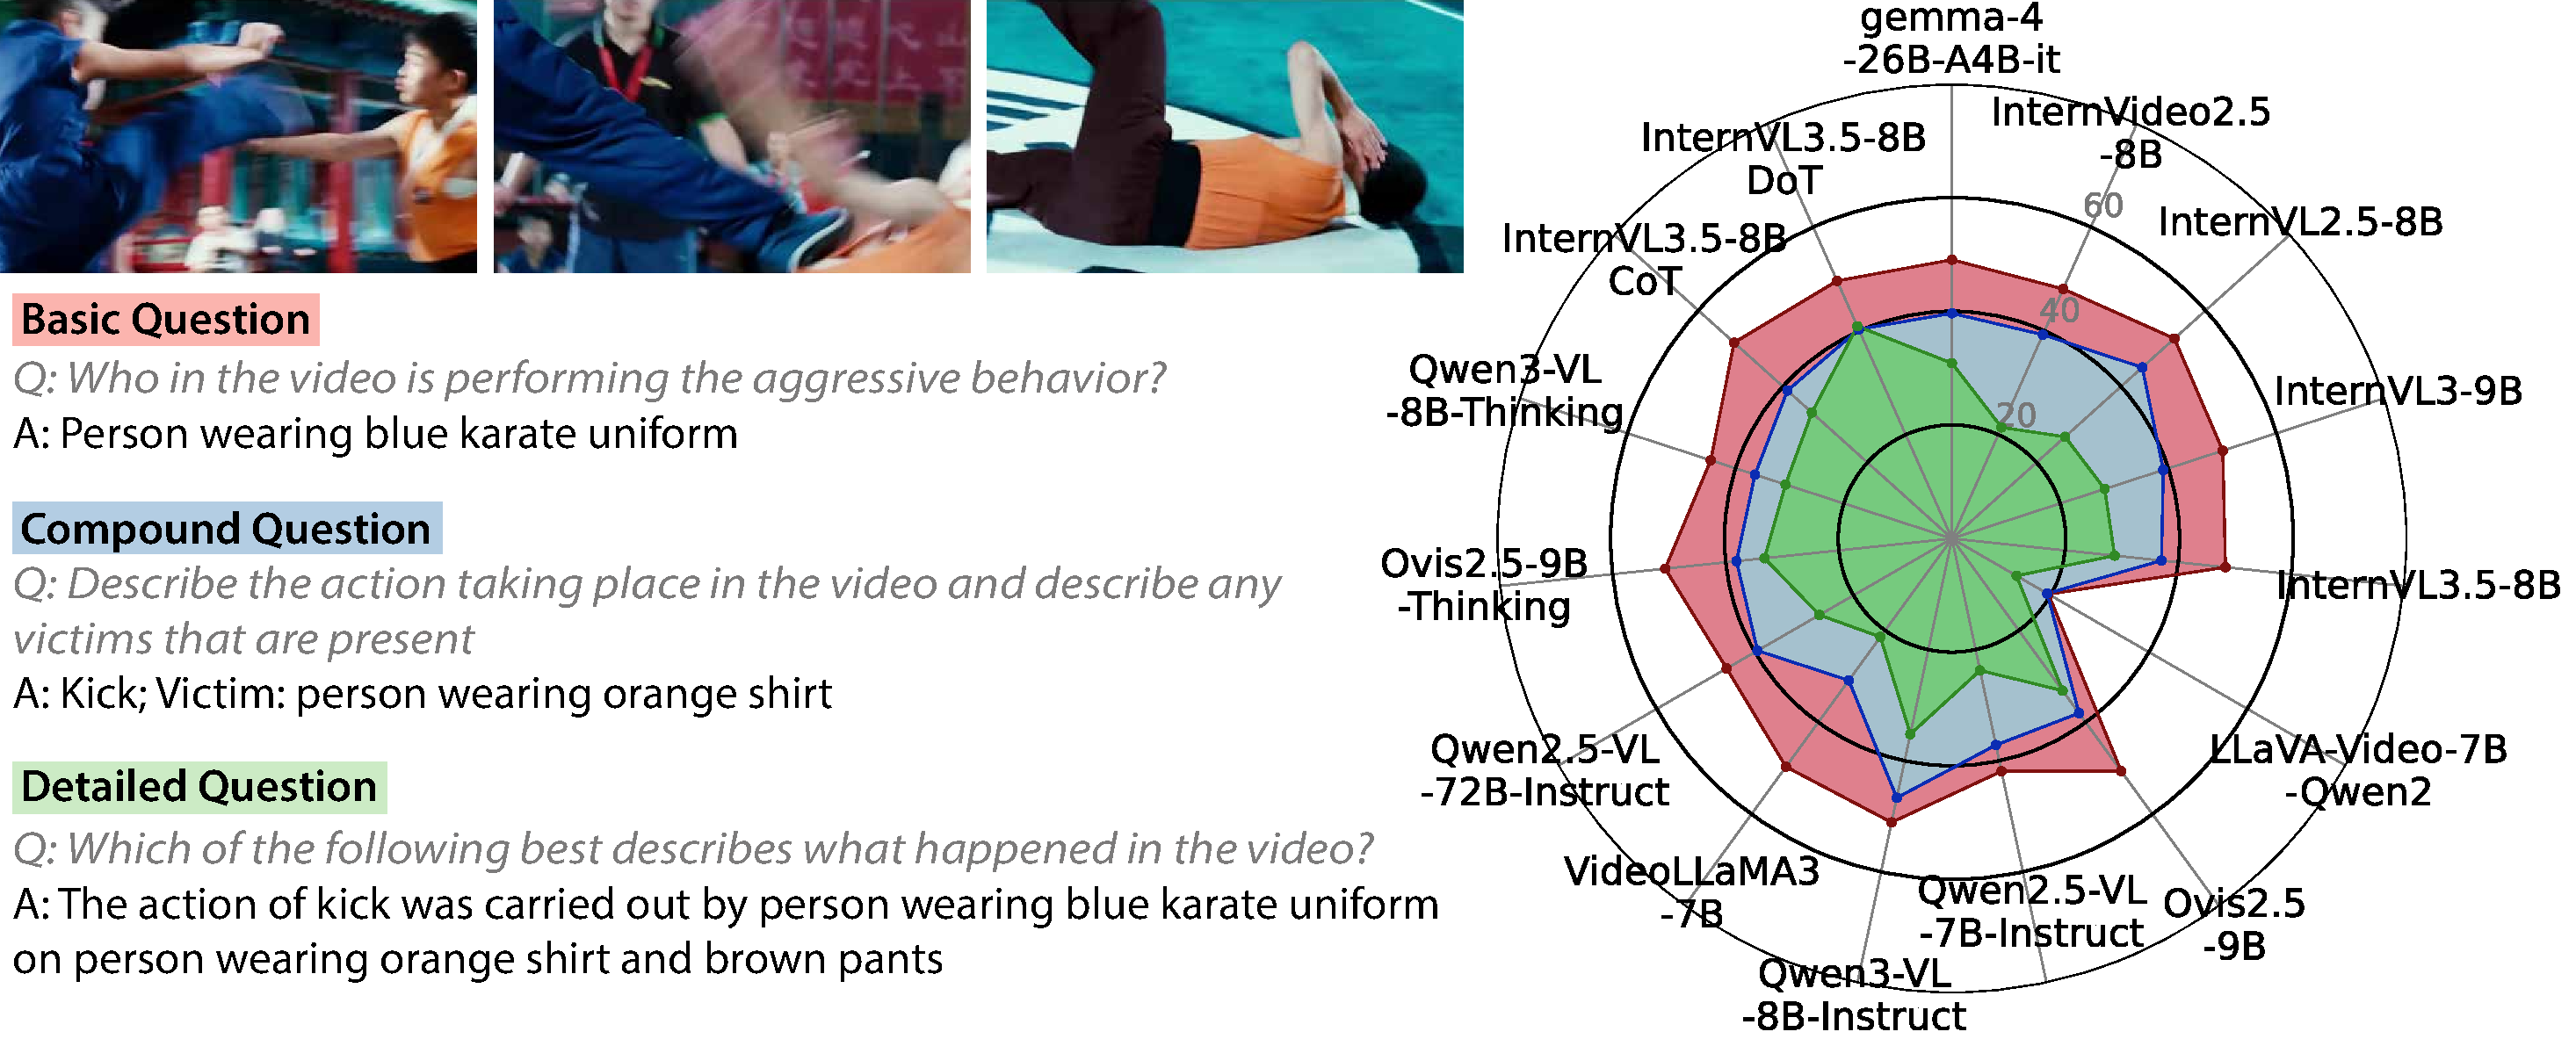
\includegraphics[width=\linewidth]{figures/teaser.pdf}
    
  \caption{\textbf{A$^3$Bench evaluates fine-grained aggressive action and association.}
\textit{Left:} Example question types. The benchmark progresses from basic questions that ask about a single attribute, to detailed questions that require understanding all aspects. \textit{Right:} Performance of evaluated MLLMs across the three question levels. Models perform poorly overall most scoring below 50\%, and accuracy decreases as the task becomes more difficult, with the lowest scores on detailed questions. This highlights the difficulty of moving from coarse aggression recognition to reliable actor-role and action binding.
\RA{reminder: need to update with GPT scores}
}

  \label{fig:teaser}
\end{figure}
\section{Related Work}
\noindent\textbf{Action recognition:}
The advancement of action recognition can be noted across video \cite{VideoMAE, ActionDetailLAQ}, skeleton \cite{FreqSemSkeleton, CrossModalSkeleton, skeletoncontext}, and multimodal modalities \cite{vificlip, actionclip, xclip, froster, t2l, AudioVisualLearning}. Certain methods, such as temporal localization \cite{TriDet, Stepwise, PseudoFormer} allow more precise event boundary detection. Fine-grained recognition has advanced through unified keypoint-based frameworks \cite{Keypoint} and atomic action decomposition \cite{Atomic}. Action detection methods further localize and identify what each person is doing in space and time, but they typically focus on individual actions rather than the relationships between interacting participants. These methods still treat actions as a classification problem over participant-agnostic categories, without modeling the relationships between those involved.

\noindent\textbf{Crime and anomaly detection:}
Anomaly detection and behavior analysis in security videos have been widely studied for identifying abnormal, unsafe, or criminal activities~\cite{OSAR,surveillancevqa}. In parallel, dedicated violence and aggression datasets have advanced the evaluation of models across diverse harmful scenarios, including fight detection, crowd violence, real-world security violence, intruder activity, child aggression, and crime/anomaly recognition~\cite{moviesfight,dvd,rlvs,violentflows,rwf,vid,iard,xdviolence,cabad,crxk,ucfcrimes}. Beyond visual understanding, text-based aggression detection has also examined aggressive behavior in language, such as harmful or hostile social-media comments~\cite{AggressiveComments}, showing that aggression analysis spans multiple modalities. Most existing video benchmarks focus on violence, aggression, or anomaly detection with coarse event-level labels. In contrast, A$^3$Bench evaluates fine-grained aggressive action association by requiring models to identify the actor, target, and role of each visible participant, exposing failures that prior benchmarks do not measure.

\noindent\textbf{Multimodal Large Language Models (MLLMs):}
Recent multimodal models have significantly expanded the scope of visual understanding by linking visual evidence with language-based semantic reasoning~\cite{clip}. Building on large-scale cross-modal pretraining, such models have enabled zero-shot and open-vocabulary recognition of human actions and activities~\cite{VLM-WACV25,actionclip,xclip,vificlip,froster,t2l}. Recent video-centric MLLMs~\cite{qwen3vl,internvl3,ovis2_5,gemma4}, further extend these capabilities to temporal and multi-frame reasoning over complex events~\cite{VideoGPT,SeViLA,LVR}. These advances motivate the use of MLLMs for aggressive action and association, where models must not only identify the observed action but also reason about the relationships between people and their roles.

\RA{Prior solution methods (Will write this later if solution works)}


\section{Benchmarking Aggressive Action and Association}
A$^3$Bench is designed to evaluate fine-grained aggressive action and association in real-world videos. The benchmark construction begins with video curation and structured annotation of aggressive interactions, including actions, participants, roles, and scene context. These annotations are then converted into three levels of diagnostic VQA questions, ranging from basic attribute recognition to compound association and detailed aggressor-action-victim reasoning. The resulting benchmark enables controlled evaluation of MLLMs under a unified multiple-choice protocol.

\begin{table}[t]
    \small
    \centering
    \caption{\textbf{Comparison of A$^3$Bench with prior crime/violence/aggressive action benchmarks.} Cls = action categories. Roles = whether explicit semantic roles (aggressor, victim, bystander) are annotated. Desc. = natural-language person descriptions. Multi-P = multi-person annotation with distinct participants. VQA = structured video question-answer pairs.
    \AB{Draft addressing YSR's comment -- added \# Videos, \# QA, Multi-P columns and abbreviated headings. CABAD/IARD video counts need verification. Remove this note when finalized.}
    }
    \label{tab:benchmark_comparison}
    \resizebox{\textwidth}{!}{
    \begin{tabular}{lcrccccc}
     \toprule
     \textbf{Benchmark} & \textbf{Cls} & \textbf{\# Videos} & \textbf{\# QA} & \textbf{Roles} & \textbf{Desc.} & \textbf{Multi-P} & \textbf{VQA} \\
     \midrule
     DVD \cite{dvd}                  & 2  & 500   & --     & \xmark & \xmark & \xmark & \xmark \\
     Movies Fight \cite{moviesfight} & 2  & 200   & --     & \xmark & \xmark & \xmark & \xmark \\
     RLVS \cite{rlvs}               & 2  & 2,000 & --     & \xmark & \xmark & \xmark & \xmark \\
     RWF-2000 \cite{rwf}            & 2  & 2,000 & --     & \xmark & \xmark & \xmark & \xmark \\
     VID \cite{vid}                  & 2  & 3,020 & --     & \xmark & \xmark & \xmark & \xmark \\
     Violent Flows \cite{rlvs}       & 2  & 246   & --     & \xmark & \xmark & \xmark & \xmark \\
     \midrule
     CABAD \cite{cabad}              & 6  & 483   & --     & \xmark & \xmark & \xmark & \xmark \\
     CRxK \cite{crxk}               & 13 & 3,484 & --     & \xmark & \xmark & \xmark & \xmark \\
     IARD \cite{iard}                & 4  & 804   & --     & \xmark & \xmark & \xmark & \xmark \\
     UCF-Crime \cite{ucfcrimes}      & 14 & 1,900 & --     & \xmark & \xmark & \xmark & \xmark \\
     XD-Violence \cite{xdviolence}   & 7  & 4,754 & --     & \xmark & \xmark & \xmark & \xmark \\
     \midrule
     \textbf{A$^3$Bench (Ours)}      & \textbf{18} & \textbf{2,683} & \textbf{18,748} & \textbf{\cmark} & \textbf{\cmark} & \textbf{\cmark} & \textbf{\cmark} \\
     \bottomrule
    \end{tabular}
    }
\end{table}



\subsection{Construction}
\textbf{Video curation and annotation:}
We curate a benchmark of 2,683 video clips collected from diverse sources, including publicly available social-media videos, UCF-Crime~\cite{ucfcrimes}, and RWF-2000~\cite{rwf}. Source videos are trimmed into shorter clips centered on individual interactions, resulting in an average clip duration of 5.75 seconds. The videos span a wide range of recording conditions, camera viewpoints, resolutions, scene layouts, and levels of visual clutter, reflecting the heterogeneity of real-world scenarios. The final corpus contains 2,234 clips with aggressive behavior and 449 non-aggressive clips.

A group of annotators labeled each video with structured scene information. The annotations include: (1) the aggressive action being performed, selected from 17 aggressive action categories and a control ``none'' category for non-aggressive clips; a short appearance description of the (2) aggressor; (3) victim; (4) bystanders (if any) and (5) the environment or setting. As seen in Figure~\ref{fig:dataset_video_examples}, person descriptions are primarily based on clothing and coarse visual appearance, such as ``person in a dark jacket,'' while avoiding names, faces, demographic attributes, or other identifying information. This design reduces the risk of relying on sensitive attributes and focuses the benchmark on visual role and action understanding. If a certain role does not exist in the video clip, or the appearance is too ambiguous, that is left out in the annotations. More details are provided in Figure~\ref{fig:dataset_demograph} and ~\ref{fig:video_role_count}.


\textbf{Annotation quality assurance:}
We curate A$^3$Bench to ensure visually grounded and reliable annotations for aggressive interactions. Because real-world clips often include occlusion, crowds, similar-looking participants, and ambiguous roles, annotators mark roles at the appropriate specificity, using collective labels or avoiding vague person descriptions when needed. Multiple annotators verify that action labels, participant roles, and aggressor-action-victim relations are supported by observable visual evidence. Unreliable annotations were re-edited through discussion and multiple revision rounds. This process preserves the complexity of real-world footage while improving annotation accuracy and consistency.

\begin{figure}[t]
  \centering
  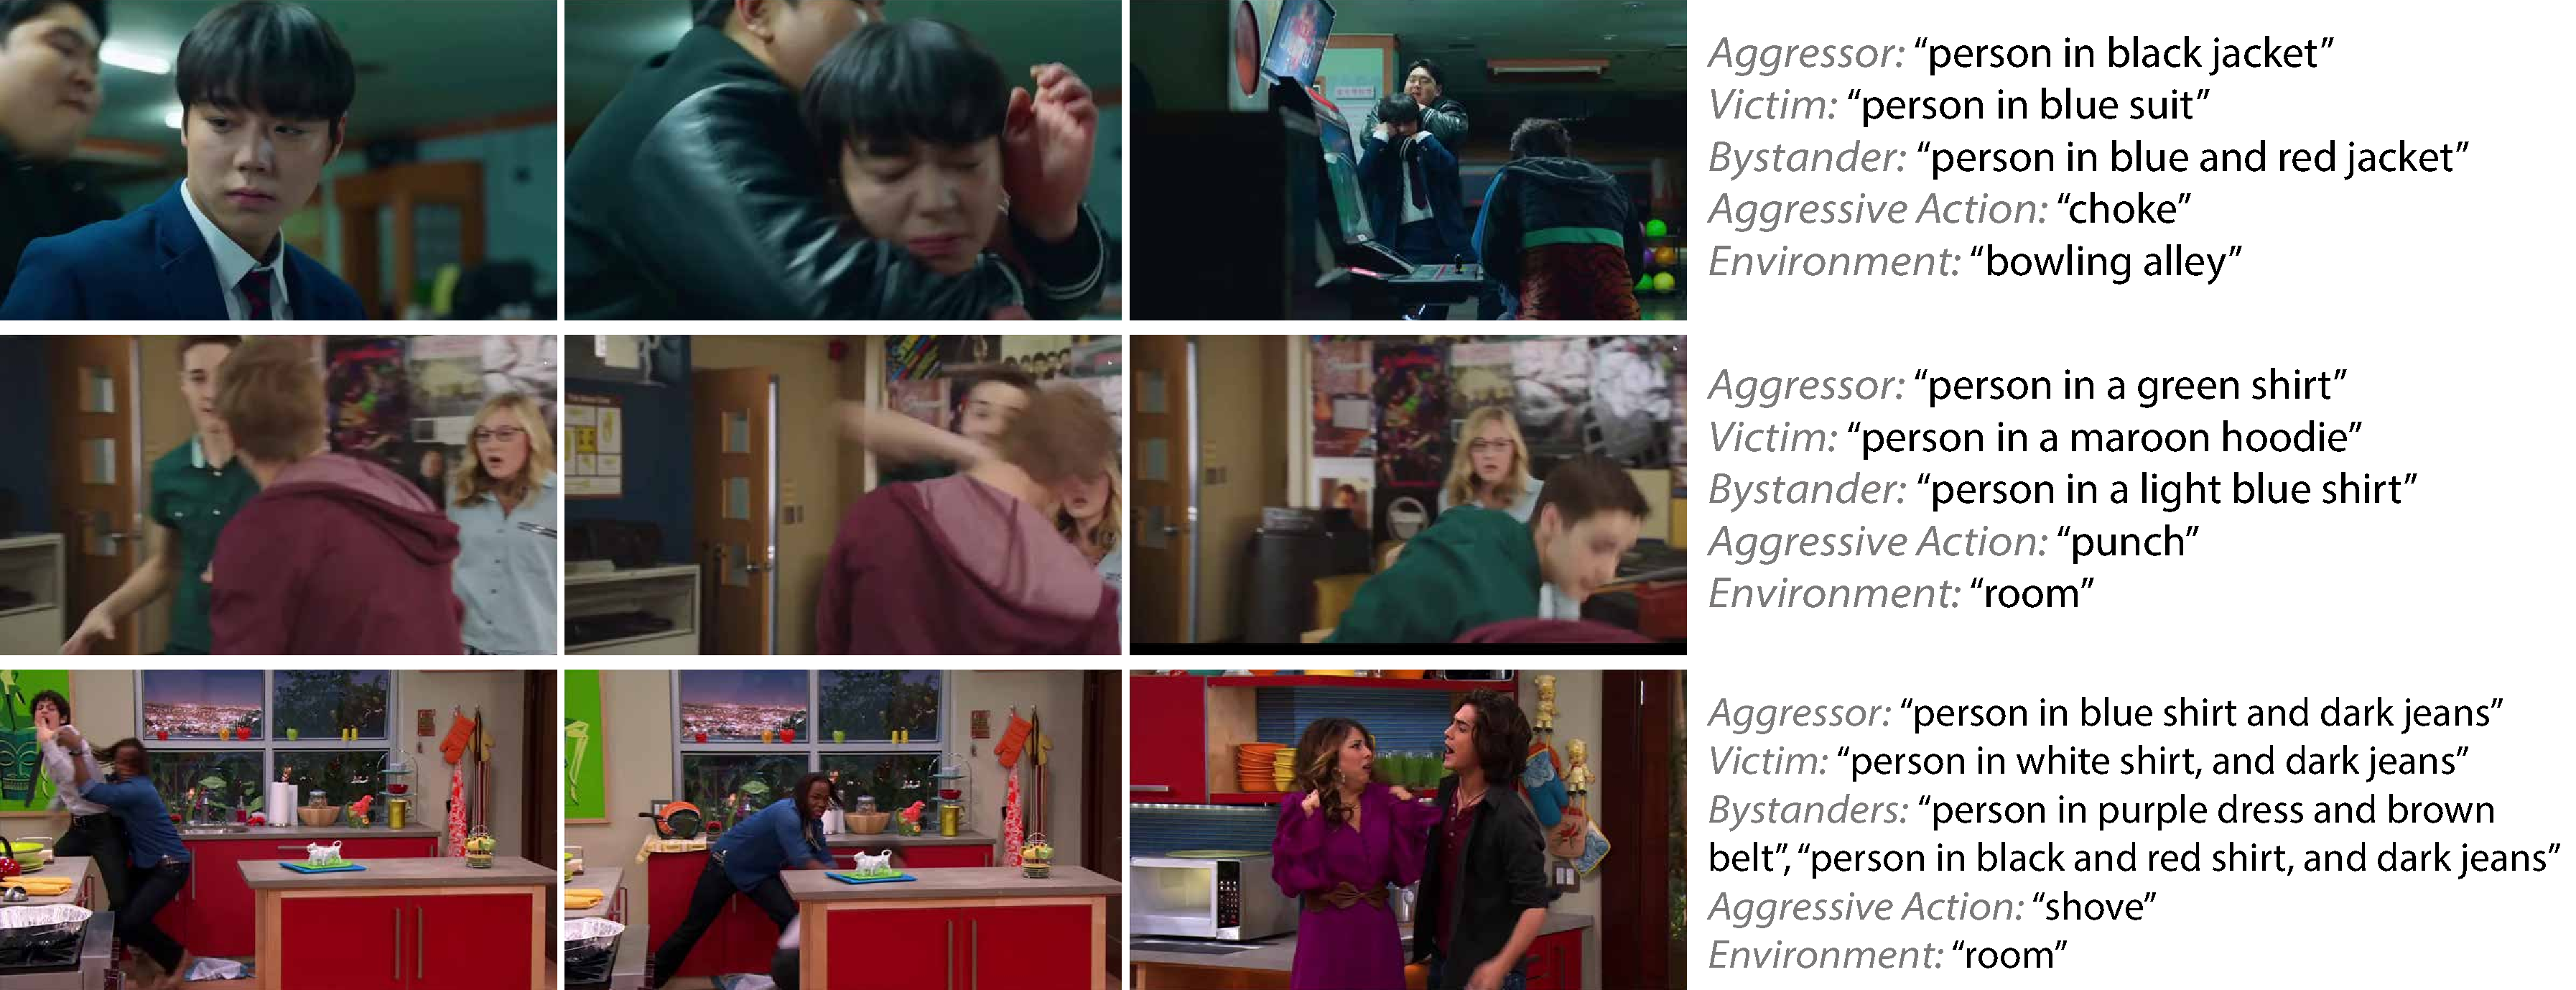
\includegraphics[width=\linewidth]{figures/dataset.pdf}
  \caption{\textbf{Example videos from A$^3$Bench.}
Each video is annotated with structured role and scene information, including the aggressor, victim, bystanders, aggressive action, and environment. Person descriptions are based primarily on clothing and coarse visual attributes rather than identity, enabling fine-grained actor-role association while avoiding personally identifying information.
}
  \label{fig:dataset_video_examples}
\end{figure}


\begin{figure}[t!]
  \centering
    \centering
    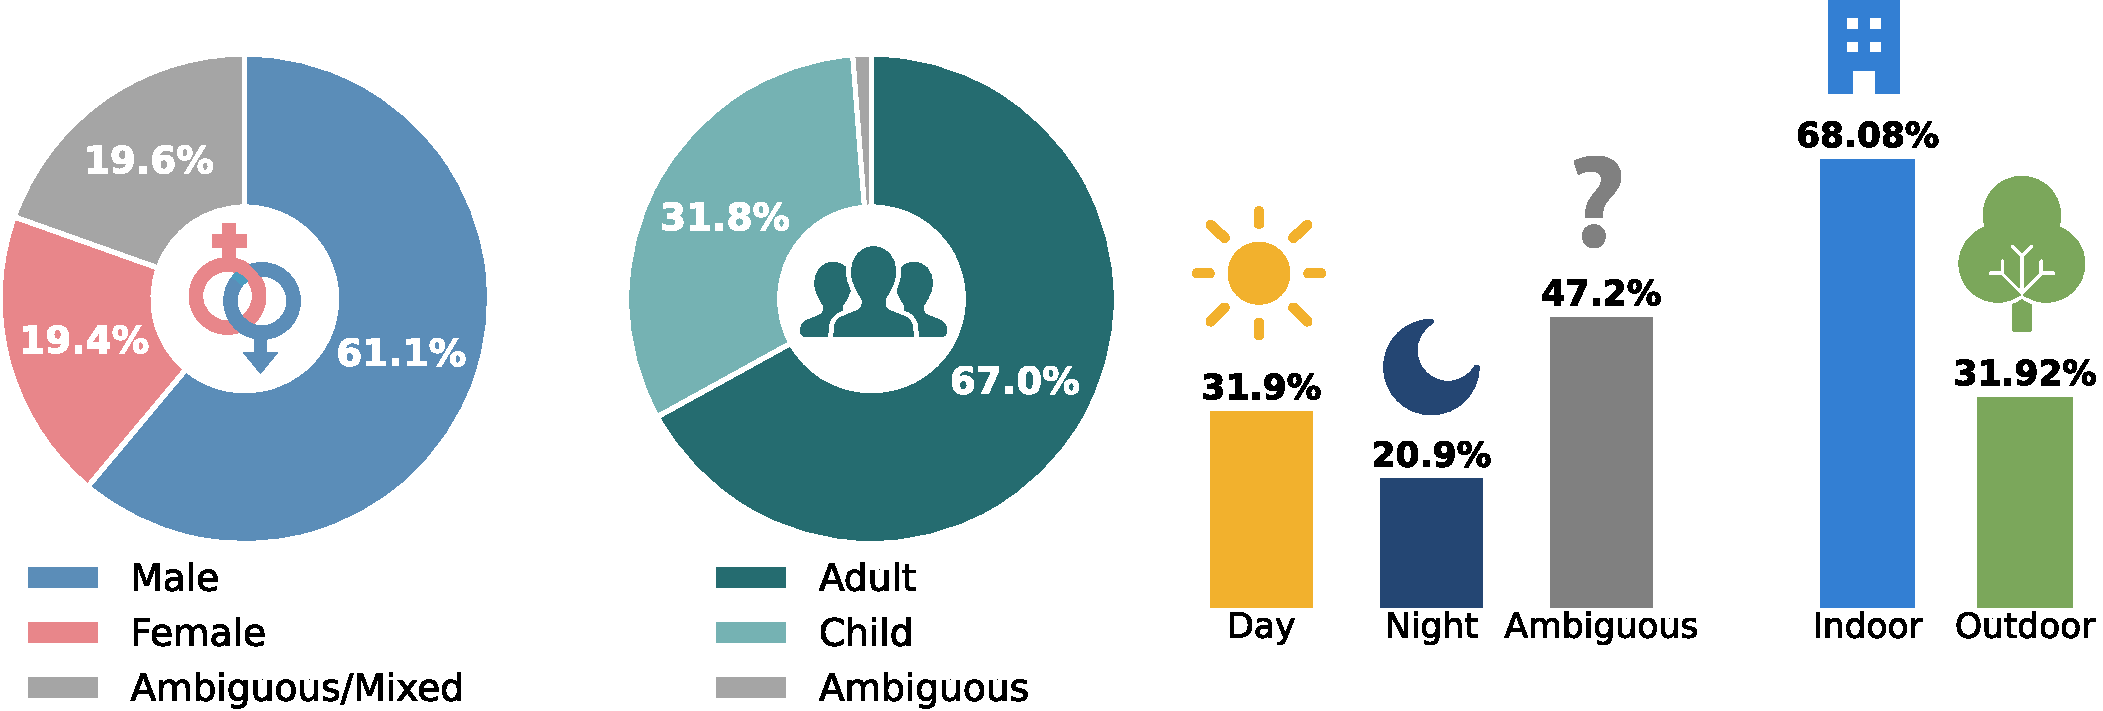
\includegraphics[width=\linewidth]{figures/dataset_demography.pdf}
    
  \caption{\textbf{Demography (aggressors and victims) and environment settings.} A$^3$Bench contains a larger proportion of male and adult participants among videos where demographic attributes are identifiable. For scene conditions, many clips are ambiguous in time of day, but among identifiable cases, slightly more aggressive clips occur during daytime than night, and most are captured in indoor environments.
}

  \label{fig:dataset_demograph}
\end{figure}

\begin{figure}[h!]
  \centering
  \begin{minipage}{0.64\linewidth}
    \centering
    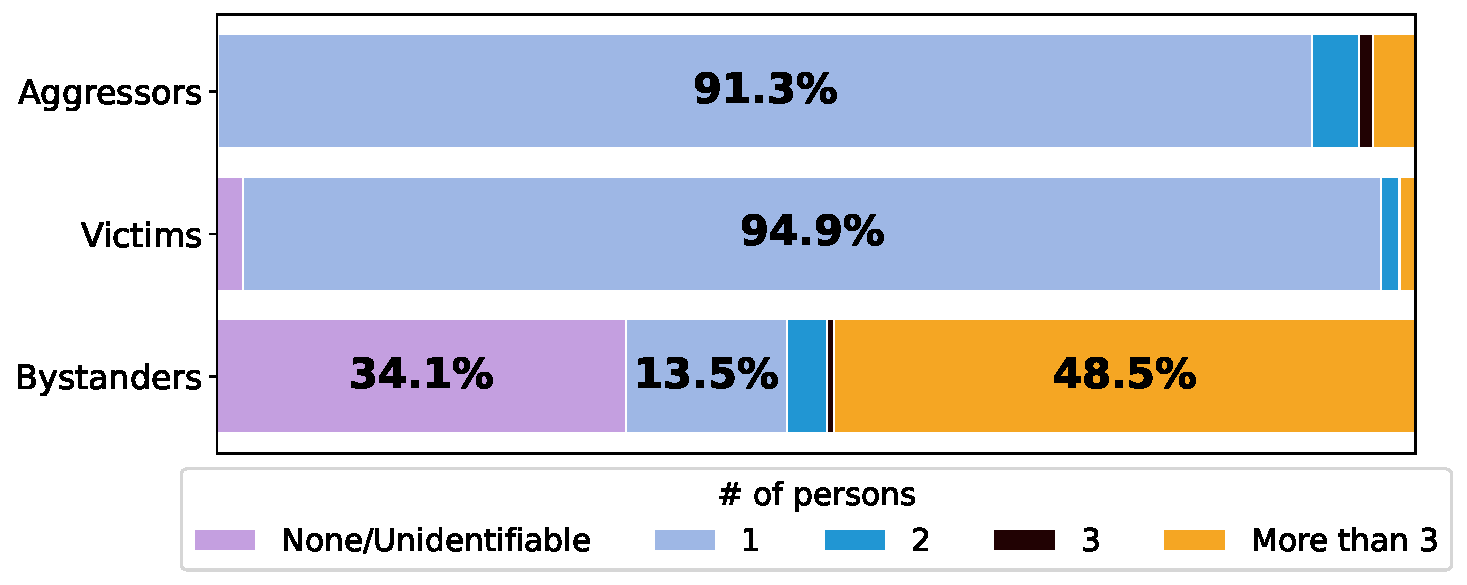
\includegraphics[width=\linewidth]{figures/role_distribution_by_video.pdf}
  \end{minipage}%
  \hfill
  \begin{minipage}{0.34\linewidth}
    \captionof{figure}{\textbf{Distribution of annotated roles per video.}
The role-count distribution is also skewed towards most clips containing a single identifiable aggressor and victim, while bystanders are more variable and often appear in larger groups.
}
    \label{fig:video_role_count}
  \end{minipage}
\end{figure}


\textbf{Question generation and distractor design:}
From the annotation corpus, we generate multiple-choice video question-answer pairs that function as controlled diagnostic probes for aggressive interaction understanding. Rather than only evaluating whether a model can recognize an action label, A$^3$Bench is designed to expose distinct failure modes in video-language models, including weak role grounding, poor action-participant binding, confusion between visible and relevant people, failure to model interaction directionality, and reliance on answer-choice priors.  The questions are organized into three tiers of increasing complexity: \textit{basic questions}, \textit{compound questions}, and \textit{detailed questions}. Figure~\ref{fig:teaser} illustrates representative examples from these three categories, and Figure~\ref{fig:question_type_category} reports their subcategories and overall distribution across the benchmark.

\textit{Basic questions} test whether a model can recover a single atomic attribute of the scene. These include primary action identification, where the model must recognize the aggressive action taking place; aggressor or victim identification, where the model must identify who performs the aggression or who is targeted; and role identification, where the model is given a person description and must assign the correct role, such as aggressor, victim, or bystander. These questions diagnose whether the model can localize individual actions and participant roles before requiring relational reasoning.

\textit{Compound questions} test whether a model can bind two scene attributes correctly. These include aggressor-victim, action-aggressor, and action-victim associations. Since each answer choice is only correct when all components are jointly correct, these questions diagnose whether models merely recognize visible actions or participants independently, or whether they can associate the correct action with the correct person and role.

\textit{Detailed questions} test whether a model can recover the full event structure of an aggressive interaction. These include aggressor-action-victim questions, which ask who did what to whom, and sequence verification questions, which require selecting the correct structured description of the interaction. These questions specifically diagnose failures in directionality, role distinction, and holistic event understanding, since a model must distinguish the aggressor from the victim and construct a coherent representation of the interaction rather than predict a participant-agnostic action category.


\begin{figure}[h!]
  \centering
  \begin{minipage}{0.64\linewidth}
    \centering
    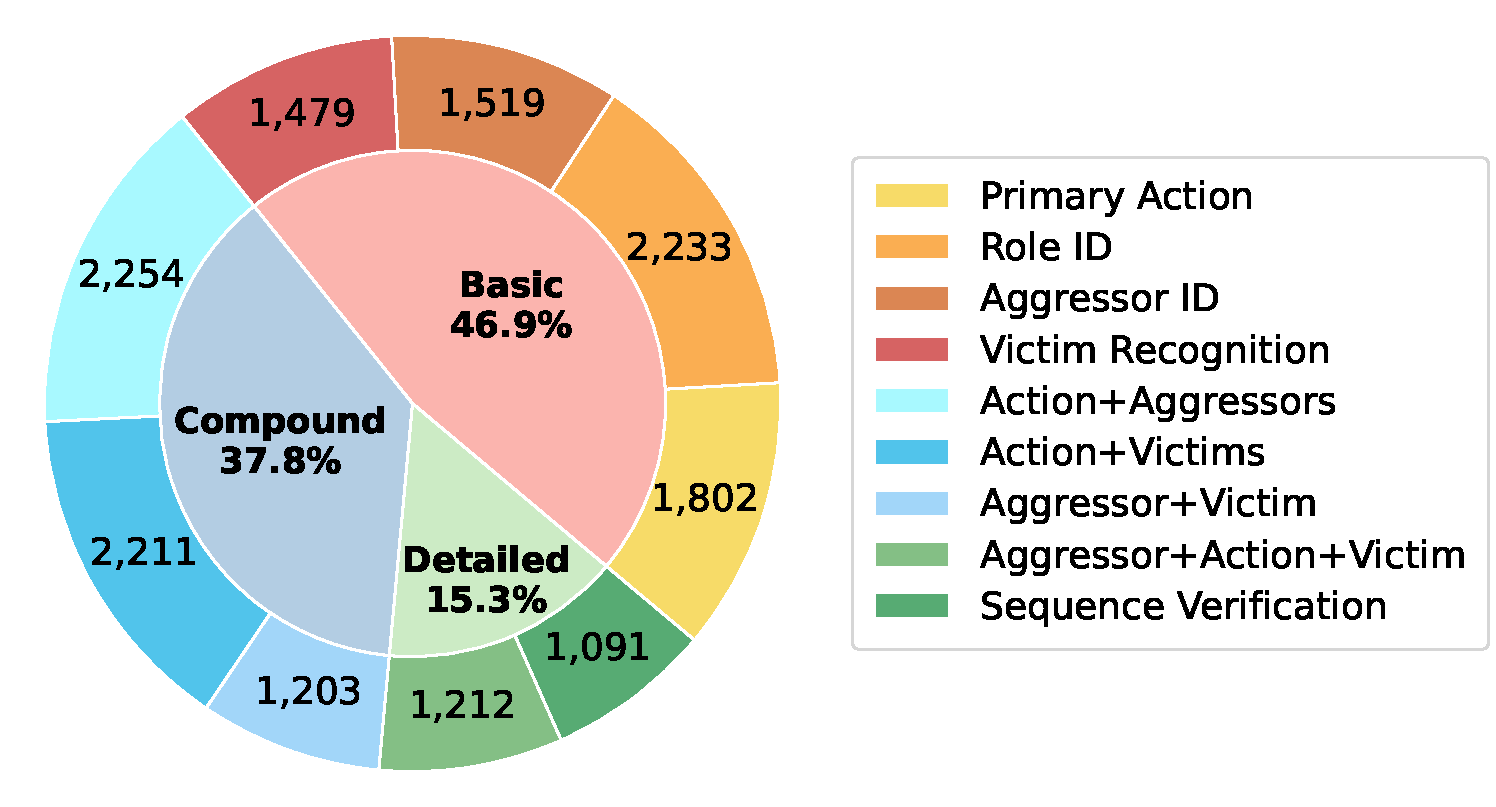
\includegraphics[width=\linewidth]{figures/category_distribution.pdf}
  \end{minipage}%
  \hfill
  \begin{minipage}{0.34\linewidth}
    \captionof{figure}{\textbf{Distribution of question types in A$^3$Bench.}
The benchmark contains three levels of questions with increasing association complexity: \textit{Basic} questions focus on single attributes; \textit{Compound} questions require associating two scene components; and \textit{Detailed} questions require full interaction understanding.
}
    \label{fig:question_type_category}
  \end{minipage}
\end{figure}


We design distractor choices as targeted diagnostic stress tests: they are visually plausible, semantically close to the correct answer, and tied to specific failure modes. \textit{Cross-video distractors} are sampled from real annotations of other clips, so incorrect options still contain natural actions, roles, and participant descriptions rather than synthetic or obviously invalid answers. \textit{Same-video distractors} use visible non-target participants from the queried clip, such as the victim or a bystander when asking for the aggressor, preventing models from relying only on visibility, saliency, or person presence. \textit{Role reversals and bystander substitutions} preserve much of the event content while swapping aggressor and victim roles or assigning bystanders to active roles, directly testing interaction directionality and the distinction between active participation and mere presence. \textit{Negation questions} include answers such as ``no aggressive action is taking place'' to test whether models verify visual evidence rather than assume aggression is present. \textit{Frequency-inverted distractors} are constructed so that each key distractor property, such as an action, role, or participant description, appears across multiple answer options, making marginal answer frequency uninformative. This forces models to reason over the complete aggressor-action-victim structure rather than selecting the option with the most common or familiar textual components.




\subsection{Benchmarked Models}

We evaluate MLLMs from \textbf{15} representative configurations on \textbf{A$^3$Bench} to assess their ability to perform aggressive action and association. All of our chosen models are trained on very large datasets with high-level video understanding. 

\noindent \textbf{General-Purpose Models.}
The evaluated models cover several recent open-weight MLLM families, including Gemma \cite{gemma4}, InternVideo \cite{internvideo2_5}, InternVL \cite{internvl2_5, internvl3, internvl3_5}, LLaVA-Video \cite{llavavideo}, Ovis \cite{ovis2_5}, Qwen-VL \cite{qwen-vl2_5, qwen3vl}, and VideoLLaMA \cite{videollama3}. These families differ in visual encoder design, video modeling strategy, instruction tuning, model scale, and reasoning behavior. 

\noindent \textbf{Reasoning and Prompted Variants.}
To investigate whether explicit reasoning improves aggressive action and association, we additionally evaluate reasoning-oriented variant of Qwen3-VL-8B \cite{qwen3vl} and enable reasoning-mode in Ovis2.5-9B \cite{ovis2_5}. We also evaluate InternVL3.5-8B \cite{internvl3_5} under two reasoning-style prompting settings: a detailed chain-of-thought (CoT) prompt and a Dream-of-Thoughts (inspired from \cite{navigatinghallucinations}) prompt. These variants encourage intermediate reasoning before producing a final answer, allowing us to test whether step-by-step inference helps models distinguish aggressors, victims, bystanders, actions, and scene context.


\subsection{Implementation Details, Evaluation Protocol, and Metrics}

All models are evaluated using their official implementations and released weights on a single NVIDIA RTX A6000 (48 GB) or A100 (80 GB) GPU. Qwen2.5-VL-72B-Instruct \cite{qwen-vl2_5} was run on the quantized version to fit in memory. We use a multiple-choice video question answering (VQA) protocol across all models: for each video-question pair, the model is prompted to select the most appropriate answer from the provided options. Depending on the question type and the size of the valid answer space, each question contains four to eight answer choices, including one correct answer and a set of diagnostic distractors. The position of the correct answer is uniformly shuffled across all questions to mitigate positional bias. This controlled evaluation setting enables fair comparison across models while directly measuring each model's ability to associate aggressive actions with the correct participants and roles. We report accuracy as the primary evaluation metric.
\YSR{no mention of train/test split?} \RA{No, since training free method, so no train set}


\begin{comment}
We also design distractor choices as targeted diagnostic stress tests. Each distractor type is constructed to be visually plausible, semantically close to the correct answer, and tied to a specific failure mode in aggressive action and association.
\begin{enumerate}
    \item \textbf{Cross-video distractors.} Incorrect answers are drawn from real annotations of other videos in the dataset. This ensures that distractors correspond to natural actions, roles, and participant descriptions rather than synthetic or obviously invalid choices. These distractors test whether models can distinguish the queried event from visually and semantically plausible alternatives.

    \item \textbf{Same-video distractors.} For person identification questions, we sample individuals with other roles who are visible in the same video. For example, when asking for the aggressor, the victim or a bystander may appear as an incorrect option. Because these individuals are genuinely present in the clip, the model cannot solve the question by simple visibility or saliency cues. This tests whether models can ground the queried role to the correct participant rather than selecting any visible person.

    \item \textbf{Role reversals and bystander substitutions.} For compound and sequence questions, we construct distractors by swapping the aggressor and victim roles. These choices preserve the same people and often the same action, but invert the relational structure of the event. This directly tests whether models understand the directionality of aggression rather than merely detecting the presence of the correct participants or action. We also place bystanders in active roles to test whether models can distinguish actual participation from mere presence in the scene.

    \item \textbf{Negation questions.} In many cases we use negation as the correct answer, such as ``no aggressive action is taking place''. These questions test whether models verify the visual evidence instead of relying on the benchmark prior that aggressive content is likely to be present. They therefore diagnose over-prediction of aggression and failure to reject unsupported relations.

    \item \textbf{Frequency-inverted distractors.} A key concern with multiple-choice evaluation is that models may exploit statistical regularities in answer text rather than ground responses in the video. To counteract such shortcuts, in Detailed questions, we use frequency-inverted distractor construction, where each distractor property appears across multiple options and marginal answer frequency is made uninformative. This forces the model to reason over the full aggressor-action-victim structure rather than selecting the option with the most common or familiar textual components.
\end{enumerate}
\end{comment}
\section{Results}
Table~\ref{tab:a3bench_results} summarizes model performance on A$^3$Bench. We report both overall accuracy, computed as the question-count-weighted average, and category average, computed as the unweighted mean across Basic, Compound, and Detailed questions. Overall, current MLLMs perform poorly on the benchmark: most models achieve below 50\% accuracy, and even the best-performing model reaches only 46.96\% overall accuracy and 44.30\% category average. These results indicate that aggressive action and association remains challenging for state-of-the-art systems. In particular, current MLLMs struggle when evaluation moves beyond coarse aggression recognition and requires identifying who is involved, what action occurs, and how participants are related.

\begin{table}[t]
\small
\centering
\caption{\textbf{Benchmarking models on A$^3$Bench.} Reported metric is accuracy (\%) for Basic Questions, Compound Questions, Detailed Questions, Overall, and Average. \textbf{Best} and \underline{second-best} performance are highlighted.
}
\label{tab:a3bench_results}
\resizebox{\textwidth}{!}{
\begin{tabular}{l | c c c c c}
\toprule
\textbf{Model}
& \textbf{Basic} \textuparrow
& \textbf{Compound} \textuparrow
& \textbf{Detailed} \textuparrow
& \textbf{Overall} \textuparrow
& \textbf{Average} \textuparrow \\
\midrule
gemma-4-26B-A4B-it \cite{gemma4} & 49.07 & 39.65 & 30.86 & 42.72 & 39.86 \\
GPT5.1 \AB{need cite} & 45.63 & 39.17 & 33.32 & 41.30 & 39.37 \\
InternVideo2.5-8B \cite{internvideo2_5} & 48.07 & 39.34 & 21.51 & 40.70 & 36.31 \\
InternVL2.5-8B \cite{internvideo2_5} & \textbf{52.61} & \underline{45.01} & 26.75 & \underline{45.77} & 41.46 \\
InternVL3-9B \cite{internvl3} & 50.05 & 39.06 & 28.22 & 42.55 & 39.11 \\
InternVL3.5-8B \cite{internvl3_5} & 48.34 & 37.03 & 28.75 & 41.06 & 38.04 \\
LLaVA-Video-7B-Qwen2 \cite{llavavideo} & 19.58 & 19.34 & 13.11 & 18.50 & 17.34 \\
Ovis2.5-9B \cite{ovis2_5} & 50.62 & 37.99 & 33.09 & 43.16 & 40.57 \\
Qwen2.5-VL-7B-Instruct \cite{qwen-vl2_5} & 41.87 & 37.15 & 23.73 & 37.30 & 34.25 \\
Qwen3-VL-8B-Instruct \cite{qwen3vl} & 51.07 & \textbf{46.65} & \underline{35.19} & \textbf{46.96} & \textbf{44.30} \\
VideoLLaMA3-7B \cite{videollama3} & 49.65 & 30.86 & 21.41 & 38.22 & 33.97 \\
Qwen2.5-VL-72B-Instruct \cite{qwen-vl2_5} & 45.73 & 39.47 & 26.91 & 40.53 & 37.37 \\
\midrule
Qwen3-VL-8B-Thinking \cite{qwen3vl} & 44.59 & 36.41 & 30.77 & 39.37 & 37.26 \\
InternVL3.5-8B CoT prompt & \underline{51.53} & 38.92 & 33.13 & 43.94 & 41.19 \\
InternVL3.5-8B DoT \cite{navigatinghallucinations} & 49.64 & 40.31 & \textbf{40.90} & 44.77 & \underline{43.62} \\
\bottomrule
\end{tabular}
}
\end{table}

\subsection{Analysis}
\textbf{Performance degrades as aggression understanding becomes more compositional.}
Models achieve an average accuracy of 47.74\% on \textit{Basic} questions, but performance drops to 38.82\% on \textit{Compound} questions and further to 29.58\% on \textit{Detailed} questions. This monotonic decline shows that current MLLMs do not simply fail at rare aggression labels; they fail progressively as the task requires role-action binding. Models can sometimes identify isolated visual cues, such as an action category, a salient participant, or a single role, but struggle once these cues must be composed into a structured interaction. \textit{Compound} questions expose failures in binding two attributes, such as linking the correct action to the correct aggressor or victim. \textit{Detailed} questions further require the full aggressor-action-victim structure, or who did what to whom. The sharp drop on these questions indicates failures in directionality, role assignment, and person-action binding.

Model-level trends show that the compositional drop is not uniform across systems. VideoLLaMA3-7B exhibits the steepest collapse, suggesting strong reliance on single-attribute cues. Qwen2.5-VL-7B-Instruct shows a small Basic-to-Compound drop but a much larger Compound-to-Detailed drop, indicating that pairwise association does not transfer to full aggressor-action-victim reasoning. Ovis2.5-9B and Ovis2.5-9B-Thinking show the reverse pattern, with larger early drops and smaller later drops, suggesting that role-action binding is their main bottleneck. Qwen3-VL-8B-Instruct achieves the strongest Compound performance but still degrades on Detailed questions, while LLaVA-Video-7B-Qwen2 remains weak across all tiers. The DoT variant is a notable exception, with Detailed accuracy slightly exceeding Compound accuracy, suggesting that structured reasoning may help complete interaction-level understanding.

%\AB{Model-wise, the drop-off rate varies dramatically. VideoLLaMA3-7B has the steepest collapse, suggesting it relies almost entirely on single-frame cues. InternVL2.5-78B degrades most gracefully in absolute terms (60.8\% to 45.8\%, -15pp) but within the InternVL2.5 family, the scale gap widens with complexity: +8.1pp at Basic but +19.0pp at Detailed, showing scale disproportionately helps compositional reasoning. In contrast, Qwen2.5-VL shows only a uniform +3pp gain from 7B to 72B across all tiers. Ovis2.5-9B is notable for holding up relatively well on Detailed (33.1\%) despite middling Basic scores (50.6\%), suggesting a different internal reasoning strategy.}

\begin{figure}[h!]
  \centering
    \centering
    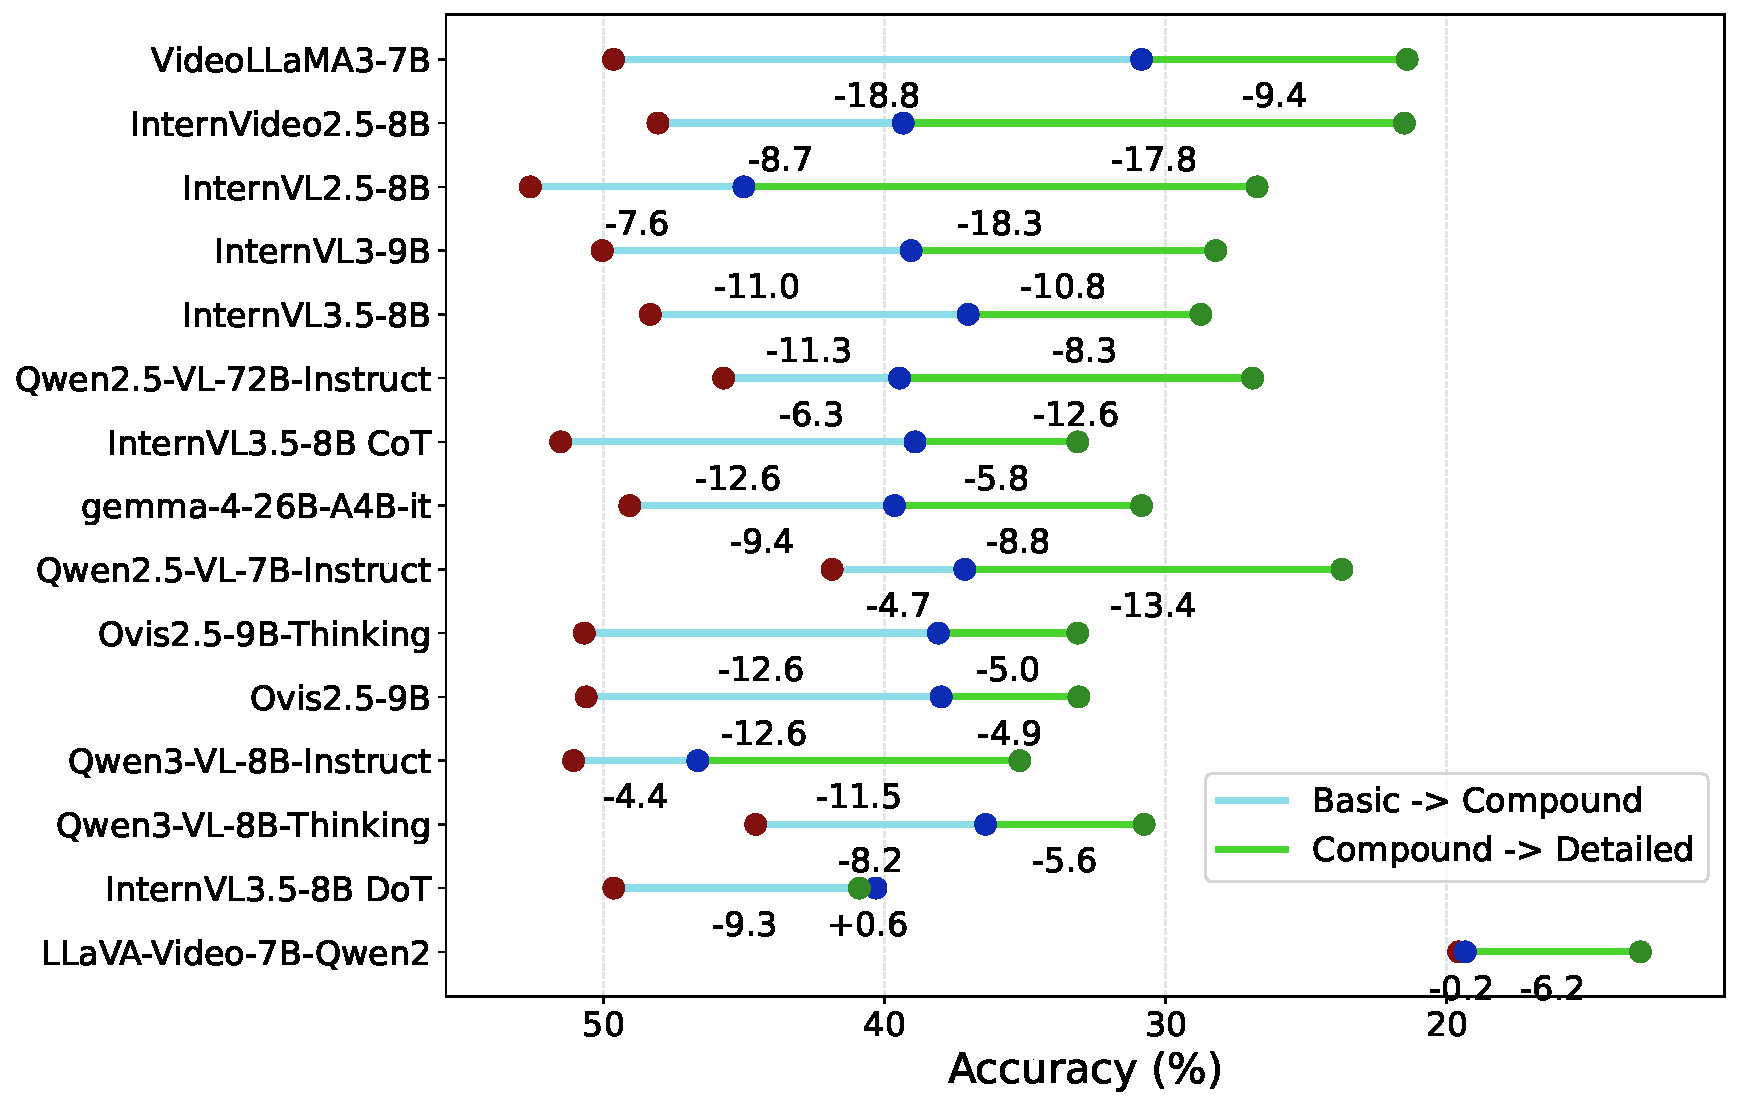
\includegraphics[width=\linewidth]{figures/scores_drop_dumbbell_plot.pdf}
    
  \caption{\textbf{Model wise drop.} \RA{keep or send to supplementary?}
}

  \label{fig:scores_drop_dumbbell_plot.pdf}
\end{figure}

\textbf{Explicit reasoning does not reliably resolve role-action association.}
Reasoning-style variants show limited gains and do not outperform the strongest general-purpose model. Their average overall accuracy remains only 42.83\%, indicating that prompting models to produce intermediate reasoning is not sufficient for reliable aggressive action and association. This suggests that the bottleneck is not only the absence of verbal reasoning, but a deeper weakness in grounding aggressive actions to the correct participants, distinguishing active roles from visible bystanders, and preserving the directionality of the interaction. \RA{Will be much shorter, we are removing ovis thinking}

% \AB{The one exception is InternVL3.5-8B-DoT (Dream of Thoughts), which achieves the flattest compositional curve of any model (49.6\% Basic to 40.9\% Detailed, only -8.7pp drop) and the second-best Detailed score (40.9\%) despite a mediocre Basic score. This is the only reasoning variant that clearly helps on the hardest questions. Qwen3-VL-8B-Thinking actually hurts: it scores 44.6\% Basic vs 51.1\% for non-thinking Qwen3, a 6.5pp regression. Ovis-Thinking is statistically identical to non-thinking Ovis (+0.08pp overall). The pattern suggests that generic ``think step-by-step'' prompting is insufficient -- the reasoning must be structured around the specific decomposition the task requires (as DoT does with its scene graph approach).}

%% 



\begin{figure}[t]
  \centering

  \begin{minipage}[t]{0.34\linewidth}
    \vspace{0pt}
    \centering

    \subcaptionbox{Action vs. role correctness\label{fig:action_vs_agg_or_victim_cm}}{
      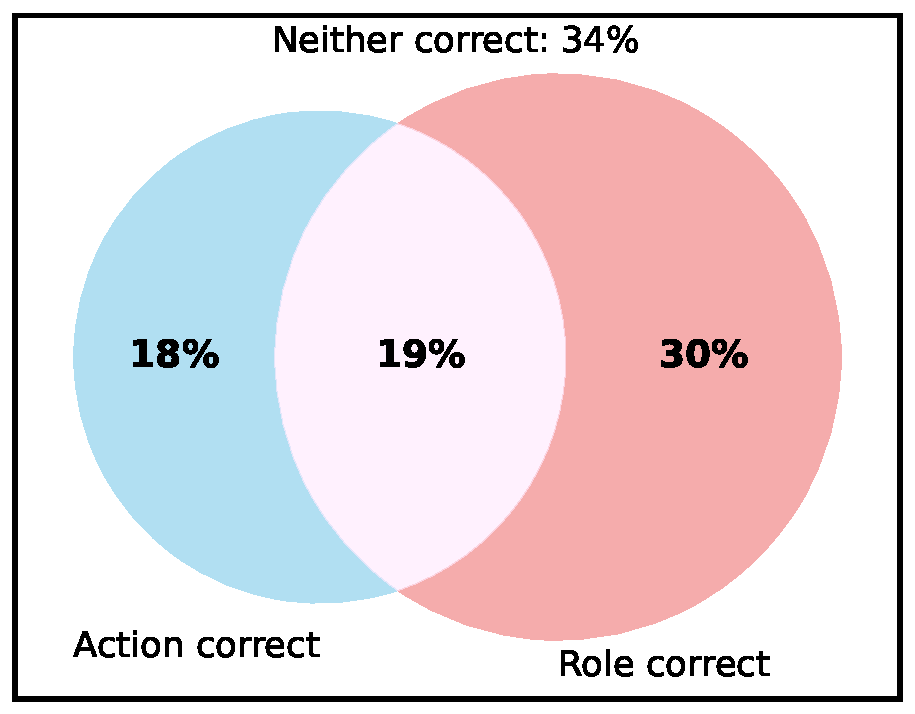
\includegraphics[width=\linewidth]{figures/calculate_action_vs_agg_or_victim_venn.pdf}
    }

    \vspace{1em}

    \subcaptionbox{Aggressor vs. victim correctness\label{fig:victim_vs_aggressor_cm}}{
      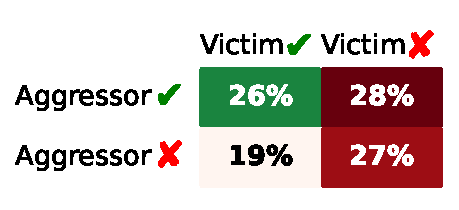
\includegraphics[width=\linewidth]{figures/calculate_victim_vs_aggressor_cm.pdf}
    }
  \end{minipage}
  \hfill
  \begin{minipage}[t]{0.64\linewidth}
    \vspace{0pt}
    \centering

    \subcaptionbox{Role identification confusion matrix\label{fig:role_confusion_matrix}}{
      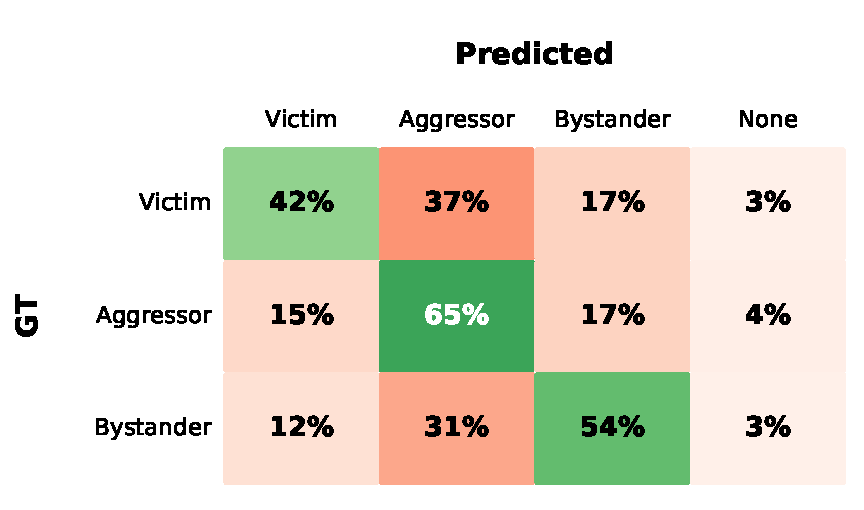
\includegraphics[width=\linewidth]{figures/role_confusion_matrix.pdf}
    }
  \end{minipage}

  \caption{\textbf{Error analysis of action and role association.}
We analyze model failures on basic questions by decomposing predictions across primary aggressive action recognition, aggressor/victim identification, and role classification. The results indicate that current MLLMs struggle not only to recognize aggressive actions, but also to assign the correct roles to the people involved.
\YSR{this is for which model? the left plots are also confusion matrix? its not clear... how about bar chart? not clear what we are showing here... make it easier for the reader..}
}
  \label{fig:error_analysis}
\end{figure}


\noindent\textbf{\textit{Models often identify participants without recognizing the correct aggressive action.}}
To understand whether errors arise from recognizing the aggressive behavior or identifying the relevant participants, we analyze videos that include both a primary action question and at least one aggressor or victim identification question. Figure~\ref{fig:error_analysis}(a) reports results averaged across models. Models are more likely to identify the correct aggressor or victim while failing to recognize the correct action (30\%) than to recognize the correct action while failing to identify the relevant role (18\%). This indicates that models may localize socially salient people in the scene, but still fail to distinguish the fine-grained aggressive action being performed. Thus, even when participant grounding partially succeeds, current MLLMs often lack reliable aggression understanding. 
\RA{discuss model wise with diagram from supplementary}

\YSR{seems like all this analysis is on average scores across all models... it will be good to also have something similar for each model... we might find some interesting pattern for each models? most of it will go in supp, but we can choose what to show here... just average across models might not be good... think about how to present it... visuals will be more dense..}

% \AB{Per-model heatmap (supplementary Figure~\ref{fig:supp_heatmap}) shows this pattern is not uniform. InternVL2.5-78B achieves 64.4\% on Aggressor ID and 54.9\% on Primary Action -- a smaller gap than most models, suggesting scale helps action recognition catch up to role detection. LLaVA-Video-7B is an outlier: it scores below 20\% on both action and role questions, so the action-vs-role decomposition does not apply -- it fails at both. VideoLLaMA3-7B has a uniquely lopsided profile: 53.9\% on Aggressor ID but only 22.6\% on Action+Aggressor compound, indicating it can sometimes locate the right person but cannot bind an action to them.}



\noindent\textbf{\textit{Models are biased toward assigning the aggressor role.}}
Figures~\ref{fig:error_analysis}(b,c) show a consistent role-grounding failure: models tend to over-assign the aggressor role when identifying participants in aggressive interactions. In Figure~\ref{fig:error_analysis}(b), when only one of the two roles is correct, models more often identify the aggressor while misidentifying the victim (28\%) than identify the victim while misidentifying the aggressor (19\%). Figure~\ref{fig:error_analysis}(c) makes this bias more explicit: a substantial fraction of ground-truth victims (37\%) and bystanders (31\%) are incorrectly predicted as aggressors. These errors suggest that models often treat visual involvement, proximity, or saliency as evidence of aggression, rather than reasoning about who initiates the action and who is targeted. As a result, they collapse distinct participant roles into a generic ``involved person'' representation, making victim and bystander grounding unreliable.

\AB{Per-model role confusion matrices (supplementary Figure~\ref{fig:supp_role_confusion}) reveal this asymmetry is extreme in some models: Ovis2.5-9B mislabels 54.3\% of true victims as aggressors, and InternVL3.5-8B reaches 47.7\%. The reverse (aggressor-to-victim) is much lower for these same models (11.0\% and 7.1\% respectively). InternVL2.5-8B shows the opposite bias: it has the worst aggressor-to-victim confusion (30.3\%) but relatively low victim-to-aggressor (17.8\%). This suggests fundamentally different internal attention strategies across architectures -- some models default to ``aggressor'' for any salient person, others distribute confusion more evenly.}

\AB{The confusion matrices make this concrete: across all models, the ``Aggressor'' column dominates predictions regardless of true role. Bystanders are classified as aggressors at rates of 30--45\% for most models (InternVL3.5-8B: 39.5\%, VideoLLaMA3: 36.5\%), meaning models treat any visible person near an altercation as a likely aggressor. LLaVA-Video-7B has a uniquely flat confusion profile -- it distributes predictions almost uniformly across all roles (20--30\% each), indicating it has no strong role prior but also no real understanding.}

\noindent\textbf{\textit{Same-video and role-reversal distractors expose weak visual grounding.}}
Distractor analysis shows that models are especially vulnerable when incorrect options are visually grounded in the same clip or preserve parts of the correct interaction structure. For Basic person-identification questions, same-video role-based distractors are more challenging than cross-video distractors because the incorrect participant is genuinely visible in the video. For Compound and Detailed questions, role-reversal distractors expose failures in directionality: models often select answers that contain the correct people and action but swap the aggressor and victim. Bystander substitutions reveal a related weakness, where models assign active roles to people who are merely present in the scene. In Detailed questions, frequency-inverted distractors further show that models may rely on answer-choice priors rather than visual grounding, selecting options with familiar or frequently co-occurring action-role-person components instead of recovering the full aggressor-action-victim structure.
\RA{Discuss from supplementary with category wise figure}

\AB{Distractor vulnerability heatmap (supplementary Figure~\ref{fig:supp_distractor}) quantifies this: role reversal causes 22--28\% of all errors across every model, confirming it is the single most effective distractor type. The vulnerability profile is strikingly uniform -- even the strongest models show the same proportional weakness to role reversal as weaker models. LLaVA-Video-7B is the one outlier with a distinctly different profile: it is much more susceptible to wrong\_aggressor (7.6\%), wrong\_victim (9.2\%), and bystander\_substitution (8.7\%) than other models (1--5\% each), confirming a broad person-identification failure rather than a directional reasoning deficit.}

\noindent\textbf{\textit{Models over-predict aggression even in non-aggressive clips.}}
We also conduct a free-form social appropriateness evaluation on five relatively strong models from the Ovis, InternVL, and Qwen families~\cite{ovis2_5, internvl2_5, qwen3vl}. Each model is asked to characterize the social appropriateness of the action shown in a video. Models are generally able to identify aggressive or socially inappropriate behavior in the 2,234 aggressive clips. However, on the 449 non-aggressive clips, they frequently still attribute inappropriate or aggressive behavior to the videos, achieving below approximately 60\% accuracy, close to random binary performance. This indicates that current models are sensitive to aggressive cues but also exhibit a strong aggression prior, over-predicting aggression even when no aggressive behavior is present.
\RA{Waiting for model scores from Austin}

\AB{Negation question analysis (supplementary Figure~\ref{fig:supp_trick}) reveals this bias varies enormously by model. InternVL3.5-8B drops 31.9pp on negation questions (47.8\% standard to 15.8\% negation -- nearly chance). InternVL3-9B and InternVL3.5-8B-CoT show similar gaps (31.1pp, 30.2pp), suggesting the InternVL3 family has a particularly strong aggression prior that reasoning prompts do not fix. In contrast, Gemma-4-26B is nearly calibrated (only 2.1pp gap, 45.7\% vs 43.6\%), and LLaVA-Video-7B actually scores slightly better on negation questions (-2.9pp gap), though both its accuracies are low. This per-model variation indicates the aggression prior is architecture-dependent, not an inherent property of the task.}

\noindent\textbf{\textit{Scene context adds another layer of grounding difficulty.}}
We further evaluate whether models can associate aggressive actions with their surrounding scene context using a subset of videos (detailed results in Supplementary) where the environment is clearly identifiable. Models are asked to identify both the action and the environment in which it occurs. Adding this scene-grounding requirement makes the task harder for most models: average accuracy drops from 40.53\% for primary action recognition to 36.69\% for action-environment association. This suggests that models are not only challenged by recognizing aggressive actions, but also by grounding those actions in the correct environmental context. While action recognition can often rely on local motion or appearance cues, action-environment association requires joint reasoning over the behavior and the broader scene.

\AB{Per the question-type heatmap (supplementary Figure~\ref{fig:supp_heatmap}), the Action+Location type averages only 36.3\% across models -- lower than most Compound types. Qwen3-VL-8B is the strongest here (46.7\%), substantially ahead of the next best. This suggests Qwen3's architecture may be better at jointly encoding spatial context with action information, possibly due to its vision encoder design or pretraining data composition.}

\YSR{this looks pretty good... great job... see if some of the above analysis can be shown as visuals/tables/etc., and less verbose... also, do we have any experiments with number of frames as input?}

\begin{comment}
\textbf{Counting}

To isolate whether models struggle with visual counting or role
assignment, we compare performance on two types of counting questions:
\emph{aggregate counts} that ask for the total number of people involved
(``how many aggressors and victims?'') and \emph{role-specific counts}
that require isolating individuals by their role (``how many
aggressors?''). This assessment was performed on the three highest achieving models 
from the benchmark test.

\begin{table}[t]
\centering
\caption{Counting accuracy (\%) on 4-option questions (chance = 25\%).
Aggregate counts require detecting people involved; role-specific counts
require assigning aggressor/victim/bystander roles first.}
\label{tab:counting}
\small
\begin{tabular}{lccc}
\toprule
Question Type & InternVL2.5-8B & Qwen3-8B & InternVL2.5-78B \\
\midrule
\multicolumn{4}{l}{\textit{Aggregate counts}} \\
\quad Aggressor + Victim     & 85.6 & 80.1 & 85.6 \\
\quad Victim + Bystander     & 94.9 & 87.9 & 95.8 \\
\midrule
\multicolumn{4}{l}{\textit{Role-specific counts}} \\
\quad Aggressor only         & 34.7 & 32.1 & 41.8 \\
\quad Victim only            & 52.2 & 52.6 & 64.2 \\
\quad Bystander only         & 26.1 & 29.9 & 17.2 \\
\midrule
Overall                      & 56.0 & 54.2 & 58.4 \\
\bottomrule
\end{tabular}
\end{table}

Models count people reliably (80--96\%) but fail when they must assign
roles first (25--42\% for aggressors and bystanders).
This confirms that role assignment --- not visual counting --- is the
bottleneck, and that counting questions probe the same capability as our
primary benchmark.
\end{comment}

\begin{comment}
We analyze this along three axes (Table~\ref{tab:text_shortcuts}). First, answer-position bias is mild: positions A--D hold the correct answer at 14.7--15.2\% versus 9.0--11.0\% for E--H, against a 12.5\% chance baseline. The elevated rate for early positions is an artifact of role identification questions, which admit only four plausible answer choices (aggressor, victim, bystander, or none) and thus concentrate correct answers in positions A--D. Second, certain negation phrases (e.g., ``no aggressive action is taking place'') appear exclusively as correct answers because they describe non-aggressive clips and cannot serve as plausible distractors elsewhere. 

Left: correct answer position distribution across 12,773 questions (chance = 12.5\%). Right: 
\begin{tabular}{c c c}
\toprule
\textbf{Pos.} & \textbf{Count} & \textbf{\%} \\
\midrule
A & 1,929 & 15.1 \\
B & 1,873 & 14.7 \\
C & 1,945 & 15.2 \\
D & 1,874 & 14.7 \\
E & 1,408 & 11.0 \\
F & 1,342 & 10.5 \\
G & 1,258 & 9.8 \\
H & 1,144 & 9.0 \\
\midrule
\textit{Chance} & & \textit{12.5} \\
\bottomrule
\end{tabular}
\hspace{8pt}

\end{comment}

\begin{comment}
Third, we directly test exploitation by comparing model accuracy when the correct answer is the most vs.\ least frequently occurring text. As shown in Table~\ref{tab:text_shortcuts}, all models achieve near-identical accuracy in both conditions (e.g., 64.3\% vs.\ 64.1\% for InternVL2.5-78B), confirming that performance reflects visual understanding rather than text-frequency pattern matching.

\begin{table}[h!]
\centering
\caption{\textbf{Text-only shortcut analysis.} model accuracy on questions where the correct answer is the most vs.\ least frequent text.}
\label{tab:text_shortcuts}
\scriptsize
\resizebox{0.5\linewidth}{!}{
\begin{tabular}{l c c c}
\toprule
\textbf{Model} & \textbf{Acc.} & \textbf{Most Freq} & \textbf{Least Freq} \\
\midrule
InternVL2.5-78B & 59.3 & 64.3 & 64.1 \\
InternVL2.5-8B & 50.3 & 63.2 & 65.4 \\
Qwen3-VL-8B & 49.9 & 61.6 & 64.5 \\
InternVL3.5-8B & 48.7 & 61.7 & 63.6 \\
Ovis2.5-9B & 48.2 & 60.8 & 65.6 \\
\bottomrule
\end{tabular}
}
\end{table}
\end{comment}
\section{Solution}
We observe that models often over-assign the aggressor role and confuse victims or bystanders with active participants. We design a role-graph prompting strategy to make the required decomposition explicit. The role graph in Figure~\ref{fig:graph_structure.pdf} is a structured formulation of aggressive-scene understanding: each visible person is first checked for physical interaction, interacting persons are then assigned an interaction direction, and roles are derived from this direction. Persons initiating contact are treated as aggressors, persons receiving contact as victims, and non-interacting persons as bystanders. The aggressive action is inferred only after the aggressor and victim are identified, encouraging the model to bind the action to the correct participants rather than relying on saliency or generic aggression cues. In implementation, we prepend this graph-based instruction template to each multiple-choice VQA query. Detailed prompt is in Supplementary.

\begin{figure}[h!]
  \centering
    \centering
    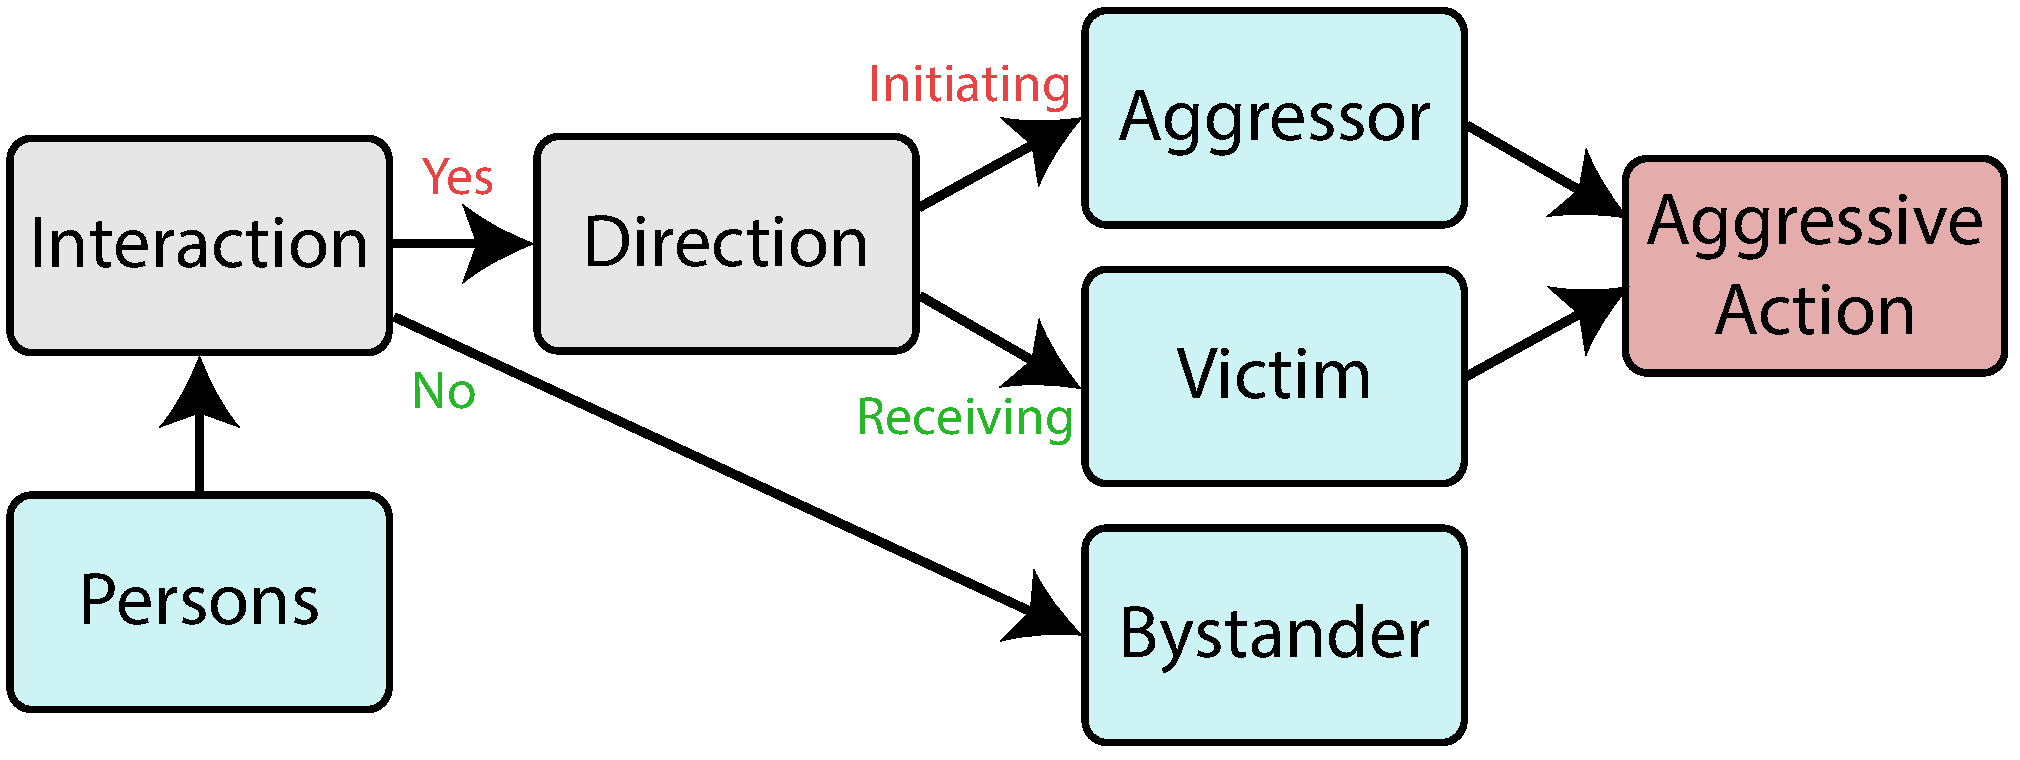
\includegraphics[width=\linewidth]{figures/graph_structure.pdf}
    
  \caption{\textbf{Graph structure?}
}

  \label{fig:graph_structure.pdf}
\end{figure}

\RA{TODO: score improvement points table}
\RA{Figure showing improvement?}
\section{Conclusion}
We presented A$^3$Bench, a benchmark of 2,683 videos and over 15K diagnostic questions designed to evaluate whether MLLMs can perform aggressive action and association -- recognizing not just that aggression occurs, but who initiates it, who is targeted, and what action connects them. Evaluation of 15 models reveals that current systems plateau below 50\% accuracy and degrade sharply as questions move from single-attribute recognition to full aggressor-action-victim reasoning. A consistent aggressor bias, in which models mislabel victims and bystanders as aggressors, persists across architectures and is not resolved by model scale or reasoning-style prompting. Our role-graph prompting strategy, which decomposes scene understanding into a structured causal chain of interaction detection, direction assignment, and role derivation, improves accuracy by up to 10 percentage points without any training, demonstrating that making the required reasoning decomposition explicit can partially compensate for the grounding deficits we identify. These results establish aggressive action and association as an open challenge for video-language models and provide a controlled diagnostic framework for measuring progress.



\begin{ack}
Use unnumbered first level headings for the acknowledgments. All acknowledgments
go at the end of the paper before the list of references. Moreover, you are required to declare
funding (financial activities supporting the submitted work) and competing interests (related financial activities outside the submitted work).
More information about this disclosure can be found at: \url{https://neurips.cc/Conferences/2026/PaperInformation/FundingDisclosure}.


Do {\bf not} include this section in the anonymized submission, only in the final paper. You can use the \texttt{ack} environment provided in the style file to automatically hide this section in the anonymized submission.
\end{ack}

{\small
\bibliographystyle{plain}
\bibliography{egbib}
}


%%%%%%%%%%%%%%%%%%%%%%%%%%%%%%%%%%%%%%%%%%%%%%%%%%%%%%%%%%%%

\appendix


\section{Supplementary material}
\RA{need to include figure examples of every question type with prompt}\\
\RA{data collection more details}\\
\RA{table for action+environment}\\
\RA{full table}\\

\begin{figure}[h!]
    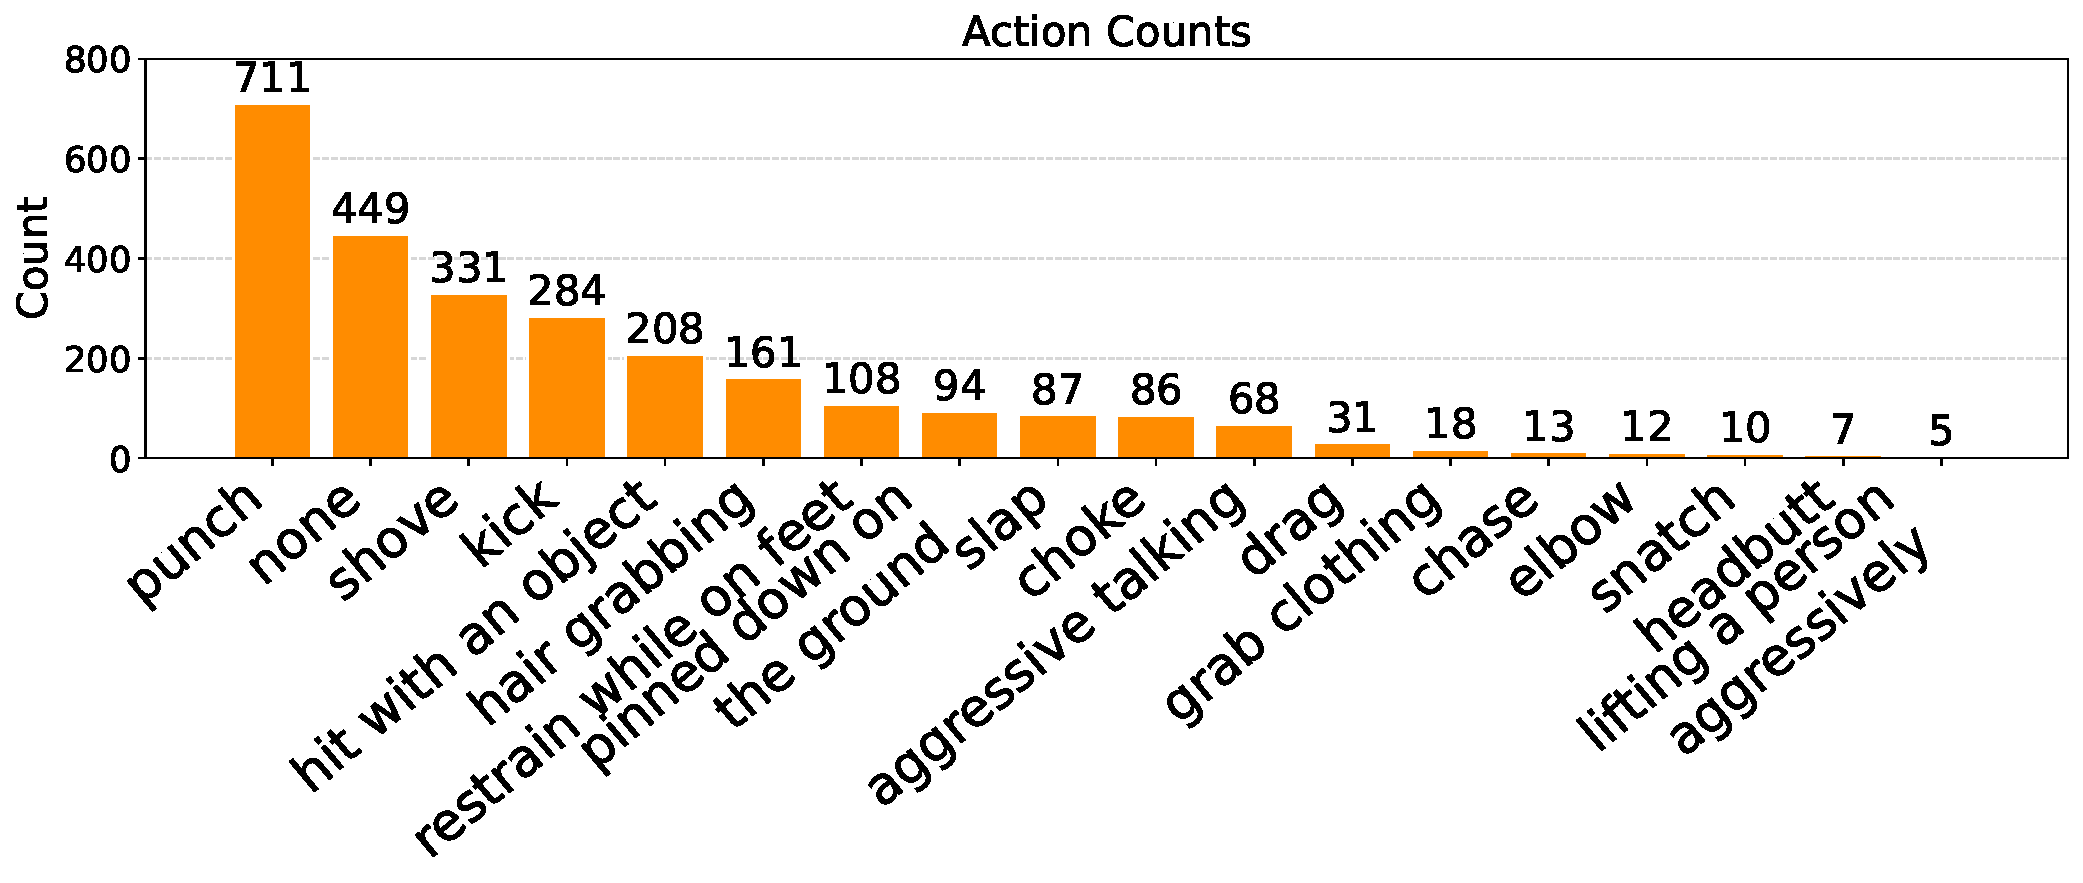
\includegraphics[width=\linewidth]{figures/action_counts.pdf}
\end{figure}

\begin{figure}[h!]
  \centering
  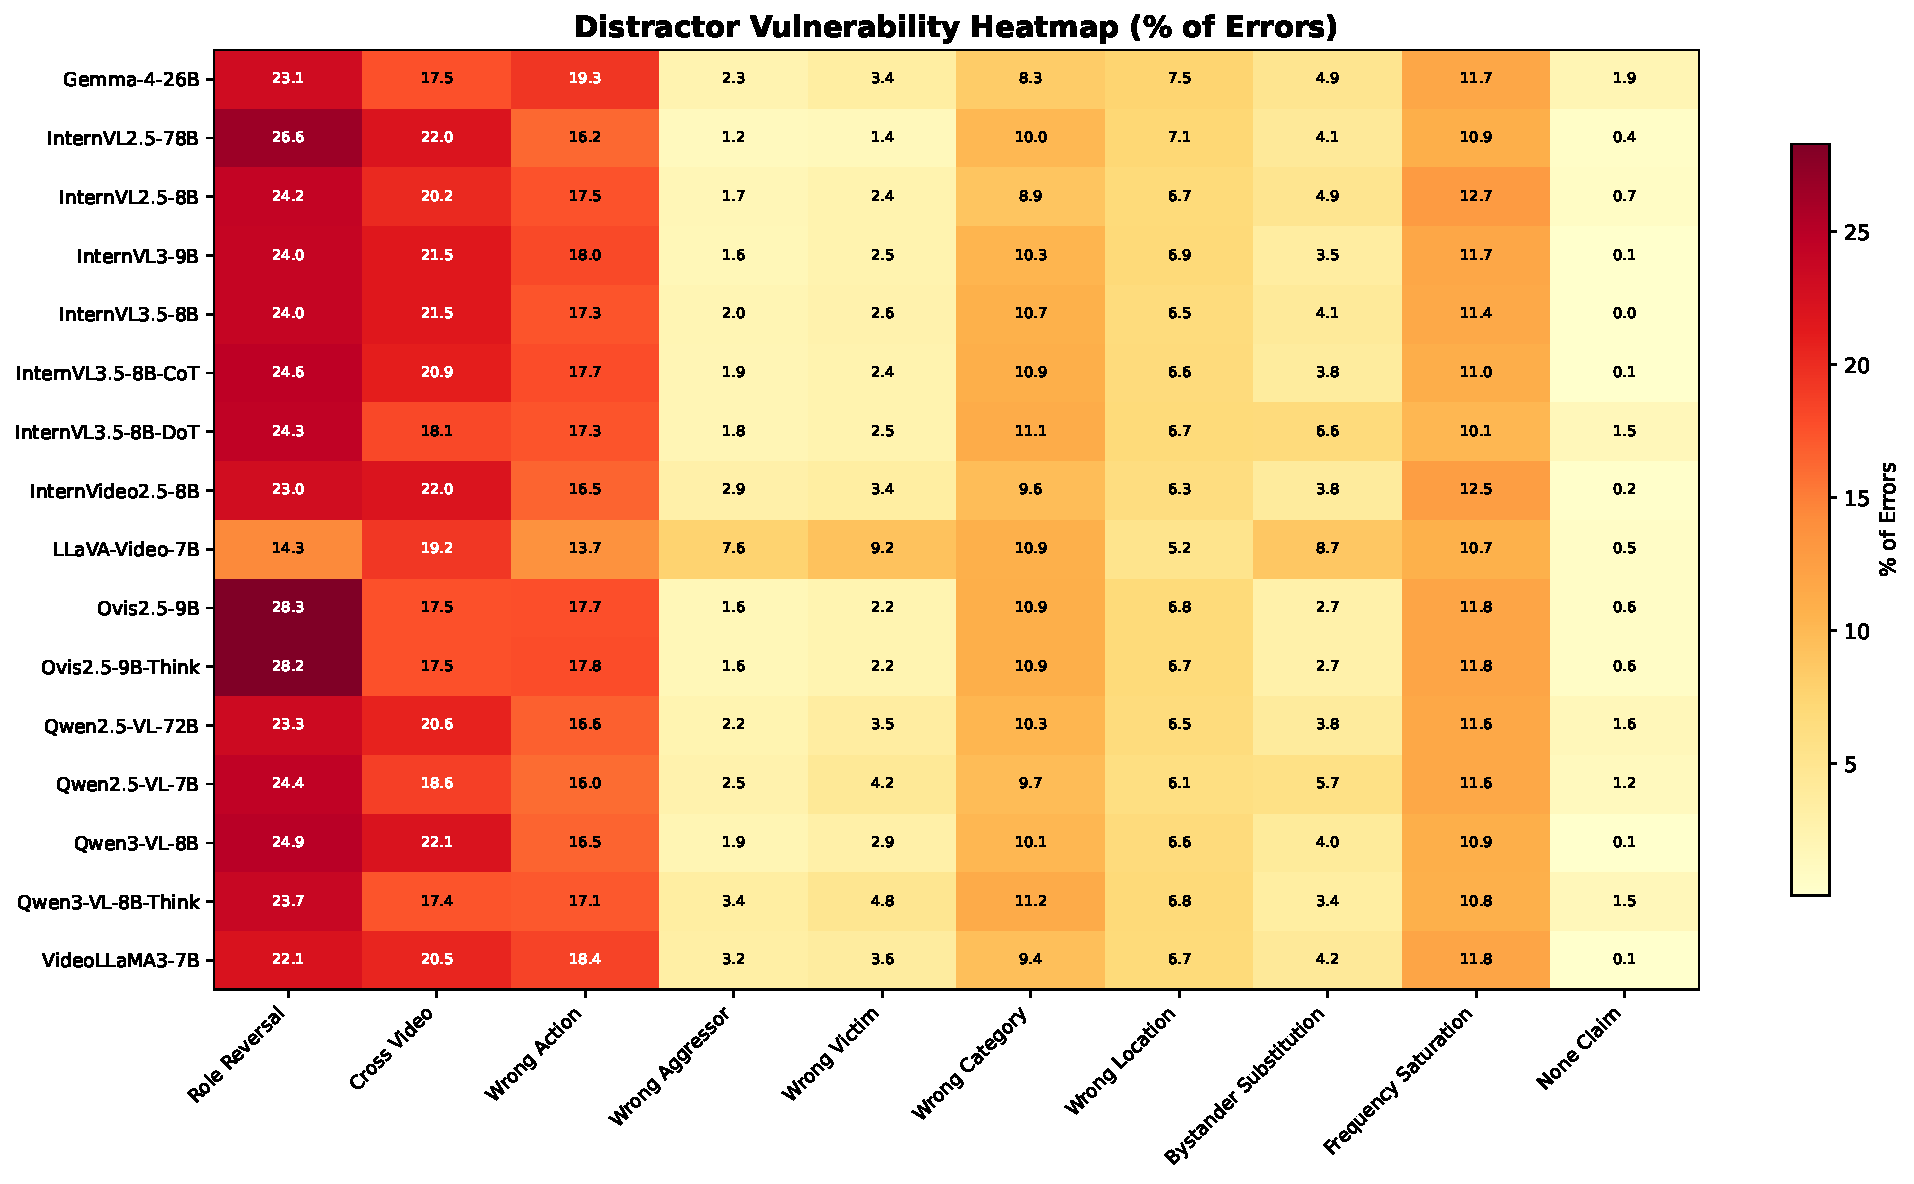
\includegraphics[width=\linewidth]{figures/distractor_vulnerability_heatmap.pdf}
  \caption{\textbf{Distractor vulnerability heatmap.} Each cell shows the percentage of a model's errors caused by each distractor type. Darker shading indicates higher vulnerability. Role reversal and cross-video distractors dominate errors across all models.}
  \label{fig:supp_distractor}
\end{figure}

\RA{full causal prompt}\\




%%%%%%%%%%%%%%%%%%%%%%%%%%%%%%%%%%%%%%%%%%%%%%%%%%%%%%%%%%%%

\newpage
\input{checklist.tex}


\end{document}